%\documentclass{book}
\documentclass{report}

\pagenumbering{roman} 
\pagestyle{empty}

% Notas de aula
%
% Template criado em 24/9/2013
% Daniel Oliveira Dantas
%
% Ctrl+x 8 , c = ç

\usepackage[utf8]{inputenc}
\usepackage[english, brazil]{babel}

\usepackage{listings}
\lstset{
  language=C,                     % choose the language of the code
  numbers=none,                   % where to put the line-numbers
  stepnumber=1,                   % the step between two line-numbers.        
  numbersep=10pt,                 % how far the line-numbers are from the code
  %backgroundcolor=\color{white}, % choose the background color. You must add \usepackage{color}
  showspaces=false,               % show spaces adding particular underscores
  showstringspaces=false,         % underline spaces within strings
  showtabs=false,                 % show tabs within strings adding particular underscores
  tabsize=2,                      % sets default tabsize to 2 spaces
  captionpos=b,                   % sets the caption-position to bottom
  breaklines=true,                % sets automatic line breaking
  breakatwhitespace=true,         % sets if automatic breaks should only happen at whitespace
  title=\lstname,                 % show the filename of files included with \lstinputlisting;
}

% Adicionado para permitir a criação de listas com vários graus de aninhamento
% ddantas, 24/03/2020
\usepackage{amssymb}
\usepackage{amsmath}
\usepackage[ampersand]{easylist}
\ListProperties(Hide=100, Hang=true, Progressive=3ex, Style*=--- ,
Style2*=$\bullet$ ,Style3*=$\circ$ ,Style4*=\tiny$\blacksquare$ )

% Adicionado para permitir a inserção de figuras
% ddantas, 24/03/2020
\usepackage{graphicx}

% Adicionado para permitir a inserção de figuras
% ddantas, 31/03/2020
\usepackage{subcaption}

%formatacao

\newcommand{\TAB}{{\hspace*{1cm}}}
\newcommand{\NEWLINE}{~\\}
\newcommand{\BV}{\begin{verbatim}}
\newcommand{\EV}{\end{verbatim}}

%tipos de dados

\newcommand{\VOID}{{\tt void}}
\newcommand{\CHAR}{{\tt char}}
\newcommand{\INT}{{\tt int}}
\newcommand{\FLOAT}{{\tt float}}
\newcommand{\DOUBLE}{{\tt double}}

\newcommand{\LONGINT}{{\tt long int}}

%operadores

%\newcommand{\AND}{{\tt \&\&}}
%\newcommand{\OR}{{\tt ||}}

%\newcommand{\LNOT}{{\tt \~{}}}
%\newcommand{\LAND}{{\tt \&}}
%\newcommand{\LOR}{{\tt |}}
%\newcommand{\LXOR}{{\tt \^{}}}

%palavras reservadas

\newcommand{\IF}{{\tt if}}
\newcommand{\ELSE}{{\tt else}}

\newcommand{\SWITCH}{{\tt switch}}
\newcommand{\CASE}{{\tt case}}

\newcommand{\FOR}{{\tt for}}
\newcommand{\WHILE}{{\tt while}}

\newcommand{\BREAK}{{\tt break}}

%\newcommand{\TRUE}{{\tt true}}
%\newcommand{\FALSE}{{\tt false}}

\newcommand{\MAIN}{{\tt main}}

\newcommand{\SIZEOF}{{\tt sizeof}}

% funcoes

\newcommand{\SIN}{{\tt sin}}
\newcommand{\COS}{{\tt cos}}
\newcommand{\TAN}{{\tt tan}}
\newcommand{\LOG}{{\tt log}}

\newcommand{\PRINTF}{{\tt printf}}
\newcommand{\SCANF}{{\tt scanf}}

\newcommand{\SPRINTF}{{\tt sprintf}}
\newcommand{\SSCANF}{{\tt sscanf}}

\newcommand{\FPRINTF}{{\tt fprintf}}
\newcommand{\FSCANF}{{\tt fscanf}}

\newcommand{\GETS}{{\tt gets}}
\newcommand{\FGETS}{{\tt fgets}}

\newcommand{\FOPEN}{{\tt fopen}}
\newcommand{\FCLOSE}{{\tt fclose}}

\newcommand{\SYSTEM}{{\tt system}}

% outros

\newcommand{\source}[1]{  \vspace{-6pt}  \caption*{ \footnotesize{Fonte: {#1}} }  }
\newcommand{\ind}{\hspace{1cm}}
\newcommand{\DFT}{\mathfrak{F}}
\newcommand{\IFT}{\mathfrak{F}^{-1}}

% lógica

\newcommand{\NOT}{\sim}
\newcommand{\OR}{\lor}
\newcommand{\AND}{\land}
\newcommand{\NAND}{\barwedge}
\newcommand{\IMP}{\rightarrow}
\newcommand{\BIC}{\leftrightarrow}
\newcommand{\DIMP}{\Rightarrow}
\newcommand{\DBIC}{\Leftrightarrow}
\newcommand{\ISINT}{\vdash}
\newcommand{\ISEM}{\vDash}
\newcommand{\TRUE}{\textit{true}}
\newcommand{\FALSE}{\textit{false}}

\newcommand{\QED}{\blacksquare}

\newcommand{\COMP}{\operatorname{comp}}

\newcommand{\SKIP}{\vspace{0.5cm}}

%renewcommand

\renewcommand\chaptername{Capítulo}
\renewcommand\lstlistingname{Listagem}
%\renewcommand\editionname{Edição}


\title{Notas de aula de Lógica para Ciência da Computação}
\author{Daniel Oliveira Dantas}
\date{11 de setembro de 2020}
\begin{document}

\maketitle

%%%%%%%%%%%%%%%%%%%%%%%%%%%%%%%%%%%%%%%%%%%%%%%%%%%%%%%%%%%%
%Índice
%%%%%%%%%%%%%%%%%%%%%%%%%%%%%%%%%%%%%%%%%%%%%%%%%%%%%%%%%%%%

\tableofcontents
\pagestyle{plain}


%%%%%%%%%%%%%%%%%%%%%%%%%%%%%%%%%%%%%%%%%%%%%%%%%%%%%%%%%%%%
%Capítulo: A linguagem da lógica proposicional
%%%%%%%%%%%%%%%%%%%%%%%%%%%%%%%%%%%%%%%%%%%%%%%%%%%%%%%%%%%%

\chapter{A linguagem da lógica proposicional}


\setcounter{page}{1}    % set page to 1 again to start arabic count
\pagenumbering{arabic}


Capítulo 1 de Souza, \textit{Lógica para Ciência da Computação}~\cite{souza_logica_3}.

\vspace{1cm}

%%%%%%%%%%%%%%%%%%%%%%%%%%%%%%%%%%%%%%%%%%%%%%%%%%%%%%%%%%%%
\begin{easylist}
  & Alfabeto: o alfabeto da Lógica Proposicional é composto por
  && Símbolos de pontuação: $( \; )$
  && Símbolos de verdade: $\TRUE \; \FALSE$
  && Símbolos proposicionais: $A \; B \; C \; P \; Q \; R \; A_1 \; A_2 \; A_3 \; a \; b \; c \; \dots$
  && Conectivos proposicionais: $ \NOT \; \OR \; \AND \; \IMP \; \BIC$

\SKIP
  
  & Fórmula: as fórmulas da linguagem da lógica proposicional são construídas a partur dos símbolos do alfabeto conforme as regras a seguir:
  && Todo símbolo de verdade é uma fórmula.
  && Todo símbolo proposicional é uma fórmula.
  && Se $H$ é fórmula, $\NOT H$ é fórmula.
  && Se $H$ e $G$ são fórmulas, $(H \OR G)$, $(H \AND G)$, $(H \IMP G)$ e $(H \BIC G)$ são fórmulas.

\SKIP
  
  & Fórmulas mal formadas: são fórmulas não obtidas da definição anterior.

\SKIP
  
  & Ordem de precedência:
  && $\NOT$
  && $\IMP \BIC$ \hspace{2cm} $A \IMP B \BIC C$ possui duas interpretações.
  && $\AND$
  && $\OR$

\SKIP
\SKIP
\SKIP
  
  & Comprimento de uma fórmula:
  && Se $H$ é um símbolo proposicional ou de verdade, $\COMP(H) = 1$.
  && Se $H$ é fórmula, $\COMP(\NOT H) = \COMP(H) + 1$.
  && Se $H$ e $G$ são fórmulas:
  &&& $\COMP(H \OR  G) = \COMP(H) + \COMP(G) + 1$.
  &&& $\COMP(H \AND G) = \COMP(H) + \COMP(G) + 1$.
  &&& $\COMP(H \IMP G) = \COMP(H) + \COMP(G) + 1$.
  &&& $\COMP(H \BIC G) = \COMP(H) + \COMP(G) + 1$.

\SKIP
  
  & Subfórmulas:
  && $H$ é subfórmula de $H$.
  && Se $H = \NOT G$, $G$ é subfórmula de $H$.
  && Se $H$ é uma fórmula do tipo $(G \OR E)$, $(G \AND E)$, $(G \IMP E)$ ou $(G \BIC E)$, então $G$ e $E$ são subfórmulas de $H$.
  && Se $G$ é subfórmula de $H$, então toda subfórmula de $G$ é subfórmula de $H$.

\end{easylist}

%%%%%%%%%%%%%%%%%%%%%%%%%%%%%%%%%%%%%%%%%%%%%%%%%%%%%%%%%%%%
%\section{Componentes de um sistema de processamento de imagens}



%%%%%%%%%%%%%%%%%%%%%%%%%%%%%%%%%%%%%%%%%%%%%%%%%%%%%%%%%%%%
%Capítulo: A semântica da lógica proposicional
%%%%%%%%%%%%%%%%%%%%%%%%%%%%%%%%%%%%%%%%%%%%%%%%%%%%%%%%%%%%

\chapter{A semântica da Lógica Proposicional}


Capítulo 2 de Souza, \textit{Lógica para Ciência da Computação}~\cite{souza_logica_3}.

\vspace{1cm}

%%%%%%%%%%%%%%%%%%%%%%%%%%%%%%%%%%%%%%%%%%%%%%%%%%%%%%%%%%%%
\begin{easylist}
  & Função: é uma relação entre dois conjuntos que associa cada elemento do conjunto de entrada a um único elemento do conjunto de saída

\SKIP
  
  & Função binária: é uma função em que seu contradomínio possui apenas dois elementos

\SKIP
  
  & Interpretação $I$ é uma função binária tal que:
  && O domínio de $I$ é constituído pelo conjunto de fórmulas da lógica proposicional.
  && O contradomínio de $I$ é o conjunto $\{T, F\}$.
  && $I(\TRUE) = T,  \; I(\FALSE) = F$.
  && Se $P$ é um símbolo proposicional, $I(P) \in \{T, F\}$.

\SKIP
  
  & Interpretação de fórmulas: dadas uma fórmula $E$ e uma interpretação $I$, o significado ou interpretação de $E$, denotado por $I(E)$, é determinado pelas regras:
  && Se $E = P$, onde $P$ é um símbolo proposicional, então $I(E) = I(P)$, onde $I(P) \in \{T, F\}$.
  && Se $E = \TRUE$,  então $I(E) = I(\TRUE)  = T$.
  && Se $E = \FALSE$, então $I(E) = I(\FALSE) = F$.
  && Seja $H$ uma fórmula, se $E = \NOT H$ então:
  &&& $I(E) = I(\NOT H) = T \DBIC I(H) = F$.
  &&& $I(E) = I(\NOT H) = F \DBIC I(H) = T$.

\SKIP

  && Sejam $H$ e $G$ duas fórmulas, se $E = (H \OR G)$ então:
  &&& $I(H) = T$ e/ou   $I(G) = T \DBIC I(E) = I(H \OR G) = T$.
  &&& $I(H) = F$ \;e\;  $I(G) = F \DBIC I(E) = I(H \OR G) = F$.
  && Sejam $H$ e $G$ duas fórmulas, se $E = (H \AND G)$ então:
  &&& $I(H) = T$ \;e\;  $I(G) = T \DBIC I(E) = I(H \AND G) = T$.
  &&& $I(H) = F$ e/ou   $I(G) = F \DBIC I(E) = I(H \AND G) = F$.
  && Sejam $H$ e $G$ duas fórmulas, se $E = (H \IMP G)$ então:
  &&& $I(H) = T$ então  $I(G) = T \DBIC I(E) = I(H \IMP G) = T$.
  &&& $I(H) = F$ e/ou   $I(G) = T \DBIC I(E) = I(H \IMP G) = T$.
  &&& $I(H) = T$ \;e\;  $I(G) = F \DBIC I(E) = I(H \IMP G) = F$.
  && Sejam $H$ e $G$ duas fórmulas, se $E = (H \BIC G)$ então:
  &&& $I(H) =    I(G) \DBIC I(E) = I(H \BIC G) = T$.
  &&& $I(H) \neq I(G) \DBIC I(E) = I(H \BIC G) = F$.

\SKIP

\end{easylist}

%%%%%%%%%%%%%%%%%%%%%%%%%%%%%%%%%%%%%%%%%%%%%%%%%%%%%%%%%%%%
%\section{Componentes de um sistema de processamento de imagens}



%%%%%%%%%%%%%%%%%%%%%%%%%%%%%%%%%%%%%%%%%%%%%%%%%%%%%%%%%%%%
%Capítulo: A sintaxe da lógica proposicional
%%%%%%%%%%%%%%%%%%%%%%%%%%%%%%%%%%%%%%%%%%%%%%%%%%%%%%%%%%%%

\chapter{Propriedades semânticas da lógica proposicional}


Capítulo 3 de Souza, \textit{Lógica para Ciência da Computação}~\cite{souza_logica_3}.

\vspace{1cm}


%%%%%%%%%%%%%%%%%%%%%%%%%%%%%%%%%%%%%%%%%%%%%%%%%%%%%%%%%%%%
\section{Propriedades semânticas}
\label{lprop:propriedadesSemanticas}

\begin{easylist}
  & Tautologia: uma fórmula $H$ é tautologia ou válida se e somente se (sse) para toda interpretação $I$ \[ I(H) = T \]

\SKIP
  
  & Satisfatibilidade: uma fórmula $H$ é satisfatível ou factível se e somente se (sse) existe pelo menos uma interpretação $I$ tal que \[ I(H) = T \]

\SKIP
  
  & Contingência: uma fórmula $H$ é uma contingência se e somente se (sse) existem interpretações $I$ e $J$ tais que \[ I(H) = T \mbox{ e } J(H) = F \]

\SKIP
  
  & Contradição: uma fórmula $H$ é contraditória se e somente se (sse) para toda interpretação $I$ \[ I(H) = F \]

\SKIP
  
  & Implicação: dadas duas fórmulas $H$ e $G$, $H \ISEM G$ ($H$ implica $G$) sse para toda interpretação $I$ \[ \mbox{ se } I(H) = T \mbox{ então } I(G) = T \]

\SKIP
  
  & Equivalência: dadas duas fórmulas $H$ e $G$, $H$ equivale a $G$ sse para toda interpretação $I$ \[ I(H) = I(G) \]

\SKIP
  
  & Dada uma fórmula $H$ e uma interpretação $I$, dizemos que $I$ satisfaz $H$ se \[ I(H) = T \]

\SKIP
  
  & Um conjunto de fórmulas $\beta = \{H_1, H_2, \dots, H_n\}$ é satisfatível sse existe interpretação $I$ tal que \[ I(H_1) = I(H_2) = \dots = I(H_n) = T \]

\SKIP

  & Um conjunto de fórmulas $\beta = \{H_1, H_2, \dots, H_n\}$ é insatisfatível sse não existe interpretação $I$ tal que \[ I(H_1) = I(H_2) = \dots = I(H_n) = T \]

\end{easylist}


%%%%%%%%%%%%%%%%%%%%%%%%%%%%%%%%%%%%%%%%%%%%%%%%%%%%%%%%%%%%
\section{Relações entre propriedades semânticas}

\begin{easylist}
  & Proposição 3.1: seja $H$ uma fórmula, \[H \text{ é tautologia } \DIMP H \text{ é satisfatível. }\]
  
  && Demonstração: $H$ é tautologia $\DBIC$
  para toda interpretação $I$, $I(H) = T \DIMP$
  existe interpretação $I$ tal que $I(H) = T \DBIC$
  $H$ é satisfatível. $\QED$

\SKIP

  & Proposição 3.3: seja $H$ uma fórmula, \[H \text{ é tautologia } \DIMP H \text{ não é contingência. }\]
  
  && Demonstração: $H$ é tautologia $\DBIC$
  para toda interpretação $I$, $I(H) = T \DBIC$
  não existe interpretação $I$ tal que $I(H) = F \DIMP$
  não existem interpretações $I$ e $J$ tais que $I(H) = F$ e $J(H) = T \DBIC$
  $H$ não é contingência. $\QED$

\SKIP

  & Proposição 3.4: seja $H$ uma fórmula, \[H \text{ é contingência } \DIMP H \text{ é satisfatível. }\]
  
  && Demonstração: $H$ é contingência $\DBIC$
  existem interpretações $I$ e $J$ tais que $I(H) = T$ e $J(H) = F$ $\DIMP$
  existe interpretação $I$ tal que $I(H) = T$ $\DBIC$
  $H$ é satisfatível. $\QED$

\SKIP

  & Proposição 3.5: seja $H$ uma fórmula, \[H \text{ é tautologia } \DBIC \; \NOT H \text{ é contraditória. }\]
  
  && Demonstração: $H$ é tautologia $\DBIC$
  para toda interpretação $I$, $I(H) = T \DBIC$
  para toda interpretação $I$, $I(\NOT H) = F \DBIC$
  $\NOT H$ é contraditória. $\QED$

\SKIP

  & Proposição 3.7: sejam $H$ e $G$ duas fórmulas, \[H \text{ equivale a } G \DBIC \; (H \BIC G) \text{ é tautologia. }\]
  
  && Demonstração: $H$ equivale a $G \DBIC$
  para toda interpretação $I$, $I(H) = I(G) \DBIC$
  para toda interpretação $I$, $I(H \BIC G) = T \DBIC$
  $(H \BIC G)$ é tautologia. $\QED$

\SKIP

  & Proposição 3.8: sejam $H$ e $G$ duas fórmulas, \[H \text{ implica } G \DBIC \; (H \IMP G) \text{ é tautologia. }\]
  
  && Demonstração: $H$ implica $G \DBIC$
  para toda interpretação $I$, se $I(H) = T$ então $I(G) = T \DBIC$
  para toda interpretação $I$, $I(H \IMP G) = T \DBIC$
  $(H \IMP G)$ é tautologia. $\QED$

% Teorema da dedução semântica.


\end{easylist}


%%%%%%%%%%%%%%%%%%%%%%%%%%%%%%%%%%%%%%%%%%%%%%%%%%%%%%%%%%%%
\section{Relações semânticas entre os conectivos da lógica proposicional}

\begin{easylist}
  & Conjunto de conectivos completo: o conjunto de conectivos $\psi$ é dito completo se é possível expressar os conectivos $\{\NOT, \OR, \AND, \IMP, \BIC\}$ usando apenas os conectivos de $\psi$.

  && O conectivo $\IMP$ pode ser expresso com $\{\NOT, \OR\}$: \[(P \IMP Q) \equiv \; (\NOT P \OR Q)\]
  && O conectivo $\AND$ pode ser expresso com $\{\NOT, \OR\}$: \[(P \AND Q) \equiv \; \NOT(\NOT P \OR \NOT Q)\]
  && O conectivo $\BIC$ pode ser expresso com $\{\NOT, \OR\}$: \[(P \BIC Q) \equiv \; \NOT(\NOT(\NOT P \OR Q) \OR \NOT(\NOT Q \OR P))\]

\SKIP

  & O conjunto $\{\NOT, \OR\}$ é completo, pois é possível expressar os conectivos $\{\NOT, \OR, \AND, \IMP, \BIC\}$ usando apenas $\{\NOT, \OR\}$.

  & Proposição 3.15 (regra da substituição): sejam $G, G', H$ e $H'$ fórmulas da lógica proposicional tais que:

  && $G$ e $H$ são subfórmulas de $G'$ e $H'$ respectivamente.
  && $G'$ é obtida de $H'$ da substituição de $H$ por $G$ em $H'$.

\[ G \equiv H \DIMP G' \equiv H' \]

\SKIP

  & Definição: o conectivo NAND $(\NAND)$ é definido por $(P \NAND Q) \equiv \; \NOT(P \AND Q)$.

  && O conectivo $\NOT$ pode ser expresso com $\{\NAND\}$: \[(  \NOT P) \equiv \; (P \NAND P)\]
  && O conectivo $\OR$  pode ser expresso com $\{\NAND\}$: \[(P \OR  Q) \equiv \; ((P \NAND P) \NAND (Q \NAND Q))\]

\end{easylist}


%%%%%%%%%%%%%%%%%%%%%%%%%%%%%%%%%%%%%%%%%%%%%%%%%%%%%%%%%%%%
\section{Formas normais na lógica proposicional}

\begin{easylist}

  & Literais: um literal na lógica proposicional é um símbolo proposicional ou sua negação.

  & Forma normal: dada uma fórmula $H$ da lógica proposicional, existe uma fórmula $G$, equivalente a $H$, que está na forma normal. Forma normal é uma estrutura de fórmula pré-definida.

  && Forma normal disjuntiva (FND): é uma disjunção ($\OR$)  de conjunções ($\AND$).
  && Forma normal conjuntiva (FNC): é uma conjunção ($\AND$) de disjunções ($\OR$).

  & Obtenção de formas normais:

  && FND:
  &&& Obtenha a tabela verdade da fórmula.
  &&& Selecione as linhas cuja interpretação é $T$.
  &&& Para cada linha selecionada, faça a conjunção ($\AND$) de todos os símbolos proposicionais cuja interpretação é $T$ com a negação dos símbolos proposicionais cuja interpretação é $F$.
  &&& Faça a disjunção ($\OR$) das fórmulas obtidas no passo anterior.

  && FNC:
  &&& Obtenha a tabela verdade da fórmula.
  &&& Selecione as linhas cuja interpretação é $F$.
  &&& Para cada linha selecionada, faça a disjunção ($\OR$) de todos os símbolos proposicionais cuja interpretação é $F$ com a negação dos símbolos proposicionais cuja interpretação é $T$.
  &&& Faça a conjunção ($\AND$) das fórmulas obtidas no passo anterior.

  \clearpage
  
  & Exemplo: encontre a FND e a FNC da fórmula $((P \IMP Q) \AND R)$.
\end{easylist}

\begin{center}
  \begin{tabular}{ c|c|c|c|c|c|c }
    $P$ & $Q$ & $R$ & $P \IMP Q$ & $(P \IMP Q) \AND R$ & FND & FNC \\
    \hline
    $T$ & $T$ & $T$ & $T$        & $T$                 & $P \AND Q \AND R$ & $ $ \\
    $T$ & $T$ & $F$ & $T$        & $F$                 & $ $ & $\NOT P \OR \NOT Q \OR      R$ \\
    $T$ & $F$ & $T$ & $F$        & $F$                 & $ $ & $\NOT P \OR      Q \OR \NOT R$ \\
    $T$ & $F$ & $F$ & $F$        & $F$                 & $ $ & $\NOT P \OR      Q \OR      R$ \\
    $F$ & $T$ & $T$ & $T$        & $T$                 & $\NOT P \AND Q \AND R$ & $ $ \\
    $F$ & $T$ & $F$ & $T$        & $F$                 & $ $ & $     P \OR \NOT Q \OR      R$ \\
    $F$ & $F$ & $T$ & $T$        & $T$                 & $\NOT P \AND \NOT Q \AND R$ & $ $ \\
    $F$ & $F$ & $F$ & $T$        & $F$                 & $ $ & $     P \OR      Q \OR      R$ \\
  \end{tabular}
\end{center}

\begin{easylist}

  && FND: $(P \AND Q \AND R) \OR (\NOT P \AND Q \AND R) \OR (\NOT P \AND \NOT Q \AND R)$
  && FNC:
    $(\NOT P \OR \NOT Q \OR      R) \AND
     (\NOT P \OR      Q \OR \NOT R) \AND
     (\NOT P \OR      Q \OR      R) \AND \\
     (     P \OR \NOT Q \OR      R) \AND
     (     P \OR      Q \OR      R)$

  
\end{easylist}




  
%%%%%%%%%%%%%%%%%%%%%%%%%%%%%%%%%%%%%%%%%%%%%%%%%%%%%%%%%%%%
\section{Exercícios}

%$ \NOT \; \OR \; \AND \; \IMP \; \BIC$

\begin{enumerate}
  \item Determine o comprimento e o conjunto de subfórmulas das fórmulas a seguir.
    \begin{enumerate}
      \item $P \OR P$
      \item $((\NOT \NOT P \OR Q) \BIC (P \IMP Q)) \AND \TRUE$
      \item $P \IMP ((Q \IMP R) \IMP ((P \IMP R) \IMP (P \IMP R)))$
      \item $((P \IMP \NOT P) \BIC \NOT P) \OR Q$
      \item $\NOT (P \IMP \NOT P)$
    \end{enumerate}
  \item Dentre as concatenações de símbolos a seguir, quais são fórmulas bem formadas e quais são fórmulas mal formadas?
    \begin{enumerate}
      \item $(P \IMP \AND \TRUE)$
      \item $(P \AND Q) \IMP ((Q \BIC P) \OR \NOT \NOT R)$
      \item $\NOT \NOT P$
      \item $\OR Q$
      \item $(P \OR Q) \IMP ((Q \BIC R))$
      \item $PQR$
      \item $A \NOT$
    \end{enumerate}

  \item Demonstre as proposições abaixo usando as regras de interpretação de fórmulas.
    \begin{enumerate}
      \item $I(P \AND Q) = T \Leftrightarrow I(\NOT(\NOT P \OR \NOT Q)) = T$
      \item $I(P \AND Q) = F \Leftrightarrow I(\NOT(\NOT P \OR \NOT Q)) = F$
      \item $I(P \AND Q) = T \Leftrightarrow I(\NOT P \OR \NOT Q) = F$
      \item $I(P \IMP Q) = F \Leftrightarrow I(\NOT P \OR Q) = F$
      \item $I(P \IMP Q) = T \Leftrightarrow I(\NOT P \OR Q) = T$
      \item $I(P \IMP Q) = F \Leftrightarrow I(P \AND \NOT Q) = T$
    \end{enumerate}
  \noindent
  Responda as questões 4, 5 e 6 conforme os exemplos abaixo.
    \begin{enumerate}
      \item Se $I(P) = F$, o que se pode concluir a respeito de $I(H)$?\\
        R: Pode-se concluir que $I(H) = T$.
      \item Se $I(P) = T$, o que se pode concluir a respeito de $I(H)$?\\
        R: Nada se pode concluir.
    \end{enumerate}
  \item Seja $H = (P \IMP Q)$ e $I$ uma interpretação.
    \begin{enumerate}
      \item Se $I(H) = T$, o que se pode concluir a respeito de $I(P)$ e $I(Q)$?
      \item Se $I(H) = T$ e $I(P) = T$, o que se pode concluir a respeito de $I(Q)$?
      \item Se $I(Q) = T$, o que se pode concluir a respeito de $I(H)$?
      \item Se $I(H) = T$ e $I(P) = F$, o que se pode concluir a respeito de $I(Q)$?
      \item Se $I(Q) = F$ e $I(P) = T$, o que se pode concluir a respeito de $I(H)$?
    \end{enumerate}
  \item Seja $I$ uma interpretação tal que $I(P \BIC Q) = T$. O que se pode concluir a respeito de
    \begin{enumerate}
      \item $I(\NOT P \AND Q)$
      \item $I(P \OR \NOT Q)$
      \item $I(Q \IMP P)$
      \item $I((P \AND R) \BIC (Q \AND R))$
      \item $I((P \OR  R) \BIC (Q \OR  R))$
    \end{enumerate}
  \item Repita o exercício anterior considerando $I(P \BIC Q) = F$.

  \item Sejam $H$ e $G$ as fórmulas indicadas a seguir. Identifique, justificando sua resposta, os casos em que $H$ implica $G$.
    \begin{enumerate}
      \item $H = (P \AND Q), G = P$
      \item $H = (P \OR  Q), G = P$
      \item $H = (P \OR \NOT Q), G = \FALSE$
      \item $H = \FALSE, G = P$
      \item $H = P, G = \TRUE$
    \end{enumerate}

  \item Demonstre as proposições abaixo ou dê um contra-exemplo.
    \begin{enumerate}
      \item Proposição 3.6: $H$ não é satisfatível $\Leftrightarrow$ $H$ é contraditória.
      \item $H$ é satisfatível $\Leftrightarrow$ $H$ não é contraditória.
      \item $\NOT H$ é tautologia $\Leftrightarrow$ $H$ é contraditória.
      \item $H$ não é tautologia $\Leftrightarrow$ $H$ é contraditória.
    \end{enumerate}
  
  \item Encontre a FND e a FNC das das fórmulas a seguir.
    \begin{enumerate}
      \item $(P \BIC Q) \AND (P \OR R)$
      \item $(P \IMP Q) \AND (P \IMP R)$
    \end{enumerate}


\end{enumerate}



%%%%%%%%%%%%%%%%%%%%%%%%%%%%%%%%%%%%%%%%%%%%%%%%%%%%%%%%%%%%
\section{Exercícios v.2}

%$ \NOT \; \OR \; \AND \; \IMP \; \BIC$

\begin{enumerate}
  \item Determine o comprimento e o conjunto de subfórmulas das fórmulas a seguir.
    \begin{enumerate}
      \item $P \OR Q$
      \item $\NOT ( P \IMP Q ) \BIC ( R \AND S)$
      \item $ (\NOT P \OR \NOT Q) \BIC \NOT ( P \AND Q )$
      \item $ ( A \AND ( B \AND ( C \AND D ) ) ) \OR ( \NOT A \AND ( \NOT B \AND ( C \AND D ) ) )$
    \end{enumerate}

  \item Dentre as concatenações de símbolos a seguir, quais são fórmulas bem formadas e quais são fórmulas mal formadas?
    \begin{enumerate}
      \item $ P \IMP ( ( Q \IMP R ) \IMP ( ( P \IMP R ) \IMP ( P \IMP R ) ) )$
      \item $ (P \OR \IMP Q) \AND R$
      \item $ ( ( P \IMP \NOT P ) \BIC \NOT P ) \OR Q$
      \item $ P \NOT \IMP Q$
    \end{enumerate}

  \item Demonstre as proposições abaixo usando as regras de interpretação de fórmulas.
    \begin{enumerate}
      \item $I(P \IMP Q) = T \Leftrightarrow I(\NOT ( P \AND Q)) = T$
      \item $I(\NOT P \IMP \NOT Q) = T \Leftrightarrow I(\NOT (\NOT P \AND Q) = T$
    \end{enumerate}
  \noindent
  Responda as questões 4 conforme os exemplos abaixo.
    \begin{enumerate}
      \item Se $I(P) = F$, o que se pode concluir a respeito de $I(H)$?\\
        R: Pode-se concluir que $I(H) = T$.
      \item Se $I(P) = T$, o que se pode concluir a respeito de $I(H)$?\\
        R: Nada se pode concluir.
    \end{enumerate}
  \item O que se pode concluir a respeito de
    \begin{enumerate}
      \item $I(P \AND Q)$ se $I(P) = T$
      \item $I(P \AND Q)$ se $I(P) = F$
      \item $I(P \OR Q)$  se $I(Q) = T$
      \item $I(P \OR Q)$  se $I(Q) = F$
      \item $I(P \IMP Q)$ se $I(P) = T$
      \item $I(P \IMP Q)$ se $I(Q) = T$
      \item $I(P \IMP Q)$ se $I(P) = F$
      \item $I(P \IMP Q)$ se $I(Q) = F$
      \item $I(P \BIC Q)$ se $I(P) = T$
      \item $I(P \BIC Q)$ se $I(P) = F$
    \end{enumerate}

  \item Mostre se os conjuntos de fórmulas a seguir são satisfatíveis ou insatisfatíveis.
    \begin{enumerate}
      \item $\{ (P \AND Q), (P \OR Q) \}$
      \item $\{ (P \AND Q), (P \IMP Q) \}$
      \item $\{ (P \OR Q),  (P \BIC Q) \}$
      \item $\{ (P \AND Q), (P \IMP \NOT Q) \}$
    \end{enumerate}

  \item Demonstre as proposições abaixo ou dê um contra-exemplo.
    \begin{enumerate}
      \item $H$ é satisfatível $\Leftrightarrow \NOT H$ é satisfatível
      \item $H$ é contraditória $\Leftrightarrow \NOT H$ é tautologia
      \item $H$ é tautologia $\Leftrightarrow \NOT H$ é contraditória
      \item $H$ é tautologia $\Rightarrow H$ é satisfatível
      \item $H$ implica $G \Leftrightarrow ( H \IMP G )$ é tautologia
      \item $H$ equivale a $G \Leftrightarrow ( H \BIC G )$ é tautologia
    \end{enumerate}

  \item Demonstre se as fórmulas a seguir são tautologias usando o método da tabela verdade e o da árvore semântica.
    \begin{enumerate}
      \item $H = ( P \OR Q ) \BIC (\NOT P \IMP Q )$
      \item $H = \NOT ( P \BIC Q ) \BIC (\NOT P \BIC Q )$
      \item $H = (\NOT P \BIC \NOT Q ) \BIC \NOT ( P \BIC \NOT Q )$
      \item $H = ( P \OR \NOT Q ) \BIC ( \NOT P  \IMP \NOT Q )$
    \end{enumerate}

  \item Demonstre por absurdo se as fórmulas a seguir são ou não tautologias.
    \begin{enumerate}
      \item $( P \AND Q ) \BIC (\NOT P \OR Q )$
      \item $( P \OR Q ) \BIC (\NOT P \OR Q )$
      \item $( P \AND Q ) \BIC ( P \AND \NOT P )$
    \end{enumerate}

\end{enumerate}

  
  

  



%%%%%%%%%%%%%%%%%%%%%%%%%%%%%%%%%%%%%%%%%%%%%%%%%%%%%%%%%%%%
%Capítulo: Métodos semânticos de dedução na lógica proposicional
%%%%%%%%%%%%%%%%%%%%%%%%%%%%%%%%%%%%%%%%%%%%%%%%%%%%%%%%%%%%

\chapter{Métodos semânticos de dedução na lógica proposicional}


Capítulo 4 de Souza, \textit{Lógica para Ciência da Computação}~\cite{souza_logica_3}.

\vspace{1cm}


%%%%%%%%%%%%%%%%%%%%%%%%%%%%%%%%%%%%%%%%%%%%%%%%%%%%%%%%%%%%
\section{Introdução}

\begin{easylist}
  & Validade de fórmulas: uma fórmula é válida sse todas as suas interpretações são iguais a $T$.
\end{easylist}


%%%%%%%%%%%%%%%%%%%%%%%%%%%%%%%%%%%%%%%%%%%%%%%%%%%%%%%%%%%%
\section{Método da tabela verdade}

\begin{easylist}
  & Método da tabela verdade: é um método exaustivo, ou seja, enumera todas as possibilidades. A desvantagem é que, se houver muitos símbolos proposicionais, a tabela fica muito grande.
  & Exemplo: seja $H = \; \NOT(P \AND Q) \BIC (\NOT P \OR \NOT Q)$, demonstre que $H$ é uma tautologia usando o método da tabela verdade.  
\end{easylist}

\begin{center}
  \begin{tabular}{ c|c|c|c|c|c|c|c }
    $P$ & $Q$ & $\NOT P$ & $\NOT Q$ & $(P \AND Q)$ & $\NOT(P \AND Q)$ & $(\NOT P \OR \NOT Q)$ & $H$ \\
    \hline
    $T$ & $T$ & $F$      & $F$      & $T$          & $F$              & $F$                   & $T$ \\
    $T$ & $F$ & $F$      & $T$      & $F$          & $T$              & $T$                   & $T$ \\
    $F$ & $T$ & $T$      & $F$      & $F$          & $T$              & $T$                   & $T$ \\
    $F$ & $F$ & $T$      & $T$      & $F$          & $T$              & $T$                   & $T$ \\
  \end{tabular}
\end{center}

%%%%%%%%%%%%%%%%%%%%%%%%%%%%%%%%%%%%%%%%%%%%%%%%%%%%%%%%%%%%
\section{Método da negação ou absurdo}

\begin{easylist}
  & Método da negação ou absurdo: funciona da seguinte maneira.
  && Faça uma suposição.
  && Se todas as substituições possíveis levarem a contradições, a suposição é falsa. Ou seja, a negação da suposição é verdadeira.

  & Exemplo: seja $H = \; ((P \IMP Q) \AND (Q \IMP R)) \IMP (P \IMP R)$, demonstre por absurdo que $H$ é uma tautologia.
  && Demonstração: assuma por absurdo que existe interpretação $I$ tal que $I(H) = F$.

  Então $I((P \IMP Q) \AND (Q \IMP R)) = T$ e
  $I(P \IMP R) = F$.

  Como $I(P \IMP R) = F$, então $I(P) = T$ e $I(R) = F$.

  Distribuindo na fórmula os valores de verdade encontados, temos

$    (( P \IMP Q) \AND (Q \IMP R)) \IMP (P \IMP R)    $

$ \;\;\;    T \hspace{30pt} T \hspace{30pt} F \hspace{10pt} F \;\;\; T \; F \; F  $

de onde obtemos

$    (( P \IMP Q) \AND (Q \IMP R)) \IMP (P \IMP R)    $

$ \;\;\;    T \;\; T \; T \;\; T \;\; F \;\; T \;\; F \hspace{10pt} F \;\;\; T \; F \; F  $

$ \hspace{32pt} \uparrow \hspace{21pt} \uparrow $

\hspace{27pt} Absurdo

Portanto, a suposição inicial de que existe interpretação $I$ tal que $I(H) = F$ é falsa. Em outras palavras, para todo $I$, $I(H)=T$, ou seja, $H$ é tautologia.

  & Exemplo: seja $H = \; (P \IMP Q) \AND ( \NOT( \NOT P \OR Q))$, demonstre por absurdo que $H$ é uma contradição.
  && Demonstração: assuma por absurdo que existe interpretação $I$ tal que $I(H) = T$.

  Então $I(P \IMP Q) = T$ e $I( \NOT( \NOT P \OR Q) ) = T$.

  Como $I( \NOT( \NOT P \OR Q) ) = T$, então $I( \NOT P \OR Q) = F$. E portanto, $I(Q) = F$, $I(\NOT P) = F$ e $I(P) = T$.

  Distribuindo na fórmula os valores de verdade encontados, temos

$    (P \IMP Q) \AND ( \NOT( \NOT P \OR Q))    $

$ \;\;\;\;\;\;    T \hspace{20pt}                   T \;\;\; T \;\;  F \;\;  T \;\;  F \;\;  F  $

mas se $I(P) = T$, temos que $I(Q)$ precisa ser $T$ já que $I(P \IMP Q) = T$, portanto obtemos

$    (P \IMP Q) \AND ( \NOT( \NOT P \OR Q))    $

$ \; T \;\;  T \;\; T \;\;\;                      T \;\;\; T \;\;  F \;\;  T \;\;  F \;\;  F  $

$ \hspace{30pt} \uparrow \hspace{78pt} \uparrow $

\hspace{50pt} Absurdo

Portanto, a suposição inicial de que existe interpretação $I$ tal que $I(H) = T$ é falsa. Em outras palavras, para todo $I$, $I(H)=F$, ou seja, $H$ é contradição.

  & Observe que para demonstrar corretamente que uma fórmula $H$ é tautologia, é necessário chegar a um absurdo em todas as substituições possíveis. Caso alguma substituição não chegue a um absurdo, pode-se interromper a demonstração e concluir que a fórmula não é tautologia. Isso é evidente, pois, se você assume que $I(H) = F$ e não chega a um absurdo, significa que essa substituição específica faz com que $I(H)$ seja $F$ e, portanto, com que $H$ não seja tautologia. Diferentes substituições representam diferentes linhas da tabela verdade, e pode ocorrer de algumas linhas serem iguais a $T$, caso em que há absurdo, e outras linhas iguais a $F$, caso em que não há absurdo. Por isso é necessário explorar todas as substituições possíveis.  O mesmo vale para a contradição.



\end{easylist}


%%%%%%%%%%%%%%%%%%%%%%%%%%%%%%%%%%%%%%%%%%%%%%%%%%%%%%%%%%%%
\section{Método da árvore semântica}

\begin{easylist}
  & Método da árvore semântica: é um método que permite a verificação da validade de uma fórmula sem ser exaustivo. A depender da fórmula, pode ser possível obter a resposta sem verificar todas as interpretações possíveis. Este conteúdo está na primeira edição do livro de Souza \textit{Lógica para Ciência da Computação}~\cite{souza_logica_1}.

%\clearpage
  
  & Exemplo: seja $H = \; \NOT(P \AND Q) \BIC (\NOT P \OR \NOT Q)$, demonstre que $H$ é uma tautologia usando o método da árvore semântica.
\end{easylist}

\begin{center}
  \begin{tabular}{ c|cccccccccc }
        & $\NOT$ & $(P$ & $\AND$ & $Q)$ & $\BIC$ & $(\NOT$ & $P$ & $\OR$ & $\NOT$ & $Q)$ \\
    \hline
      2 &        & $T$  &        &      &        & $F$     & $T$ &       &        &      \\
    \hline
      3 & $T$    & $F$  & $F$    &      & $T$    & $T$     & $F$ & $T$   &        &      \\
    \hline
      4 & $F$    & $T$  & $T$    & $T$  & $T$    & $F$     & $T$ & $F$   & $F$    & $T$  \\
    \hline
      5 & $T$    & $T$  & $F$    & $F$  & $T$    & $F$     & $T$ & $T$   & $T$    & $F$  \\
  \end{tabular}
\end{center}

\begin{figure}[h!]
  \begin{center}
    \begin{tabular}{c}
      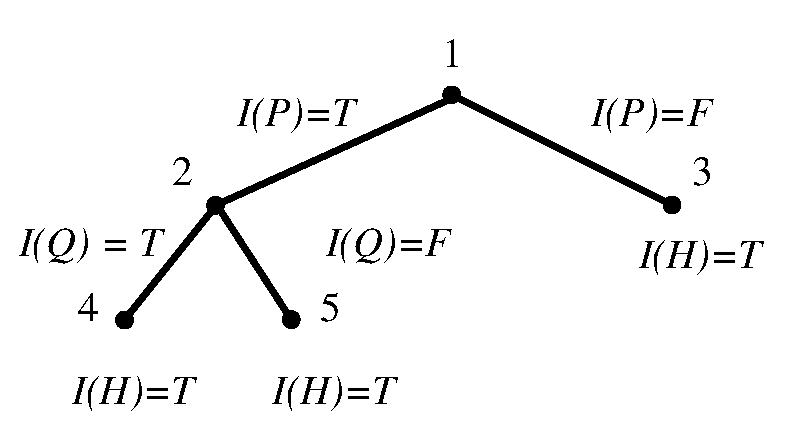
\includegraphics[width=0.7\textwidth]{images/04/tree_01.eps}
    \end{tabular}
  \end{center}
  %\caption{\label{fig:tree:01}}
\end{figure}

\clearpage

\begin{easylist}
  & Exemplo: seja $H = \; (P \OR \NOT Q) \BIC (\NOT P \IMP \NOT Q)$, demonstre que $H$ é uma tautologia usando o método da árvore semântica.
\end{easylist}

\begin{center}
  \begin{tabular}{ c|cccccccccc }
        & $(P$ & $\OR$ & $\NOT$ & $Q)$ & $\BIC$ & $(\NOT$ & $P$ & $\IMP$ & $\NOT$ & $Q)$ \\
    \hline
      2 & $T$  & $T$   &        &      & $T$    & $F$     & $T$ & $T$    &        &      \\
    \hline
      3 & $F$  &       &        &      &        & $T$     & $F$ &        &        &      \\
    \hline
      4 & $F$  & $F$   & $F$    & $T$  & $T$    & $T$     & $F$ & $F$    & $F$    & $T$  \\
    \hline
      5 & $F$  & $T$   & $T$    & $F$  & $T$    & $T$     & $F$ & $T$    & $T$    & $F$  \\
  \end{tabular}
\end{center}

\begin{figure}[h!]
  \begin{center}
    \begin{tabular}{c}
      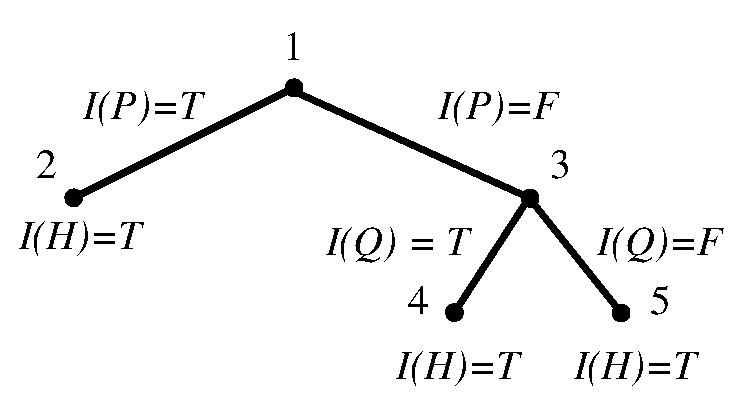
\includegraphics[width=0.7\textwidth]{images/04/tree_02.eps}
    \end{tabular}
  \end{center}
  %\caption{\label{fig:tree:01}}
\end{figure}


%%%%%%%%%%%%%%%%%%%%%%%%%%%%%%%%%%%%%%%%%%%%%%%%%%%%%%%%%%%%
\section{Método dos tableaux semânticos}

\begin{easylist}
  & Tableau semântico: sequência de fórmulas construída de acordo com um conjunto de regras e apresentada em forma de árvore. O método dos tableaux semânticos é um mecanismo de decisão para a pergunta $\beta \vdash H$, sim ou não?

  & Elementos do sistema de tableaux semânticos da lógica proposicional:
  && Alfabeto da lógica proposicional sem os símbolos de verdade $\TRUE$ e $\FALSE$.
  && Conjunto das fórmulas da lógica proposicional.
  && Um conjunto de regras de dedução.

  & Regras de dedução do tableau semântico: sejam $A$ e $B$ duas fórmulas da lógica proposicional, as regras de dedução do sistema de tableaux semânticos são

\clearpage
  
\begin{figure}[h!]
  \begin{center}
    \begin{tabular}{c}
      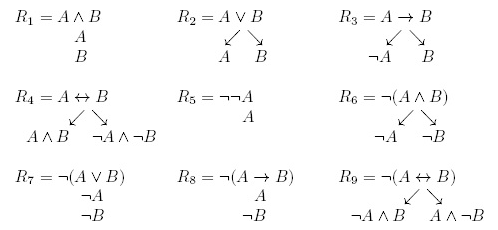
\includegraphics[width=0.7\textwidth]{images/04/tableaux.png}
    \end{tabular}
  \end{center}
  %\caption{\label{fig:tree:01}}
\end{figure}

  & Construção de um tableau semântico: se dá aplicando alguma regra de dedução uma vez para cada linha que não seja um literal (símbolo proposicional ou sua negação). O tableau resultante tende a ficar mais simples se aplicarmos primeiro as regras de dedução que não geram bifurcações $(R_1, R_5, R_7, R_8)$.
&& Exemplo: considere o conjunto de fórmulas $\beta = \{P \OR (Q \OR \NOT R), P \IMP\NOT R, Q \IMP \NOT R\}$. Verifique se $\beta \ISINT \NOT R$.

%$\beta = \{A \IMP B, \NOT(A \OR B),  \NOT (C \IMP A)\}$. Verifique se $\beta \ISINT \NOT R$.

&&& Uma possível solução seria montar a árvore semântica de $\NOT(    (P \OR (Q \OR \NOT R)) \AND (P \IMP\NOT R) \AND (Q \IMP \NOT R)  \IMP \NOT R)$.

%$\NOT (    (  (A \IMP B) \AND \NOT(A \OR B) \AND \NOT (C \IMP A)  ) \IMP \NOT R    )$.

&&& Uma solução equivalente é listar as hipóteses de $\beta$ seguidas da negação da conclusão.
%Encontre o tableau semântico iniciado com esse conjunto de fórmulas.

\end{easylist}

%\forestset{%
%  vertical/.style={                       %define style for phantom node
                                          %with vertical edge drawn from it
%    before drawing tree={not ignore edge, edge=draw},
%  },
%}

%\begin{tableau}
%  {line no sep= 1.5cm,
%    just sep= 1.5cm,
%    for tree={s sep'=10mm},
%    close with=\absurd
%}
%  [((P \land Q) \lor R),                   just={Premiss}
%    [\neg\neg(\neg P \lor \neg R),       just={Negated conclusion}
%      [(\neg P \lor \neg R),           just={From (2)}
%        [(P \land Q),                just={Alternatives from (1)}
%          [P,                      just={From (4)}
%            [Q,                  just={From (4)}
%              [\neg P,close]
%              [\neg R,         just={Alternatives from (3)}
%        ]]]]
%        [R
%          [, vertical               %phantom node but with edge
%            [, vertical       %phantom node but with edge
%              [\neg P]          %and now we have two
%              [\neg R,close]    %brances added
%  ]]]]]]
%\end{tableau}

\iffalse

\forestset{%
  vertical/.style={     %define style for phantom node
                        %with vertical edge drawn from it
    before drawing tree={not ignore edge, edge=draw},
  },
}

\begin{tableau}
{                              % begin tree preamble
    line no sep= 2cm,          % distance of tree from line numbers
    just sep= 1.5cm,
    for tree={s sep'=10mm},    % control horizontal spread of branches
}                              % end tree preamble
  [P
    [(P \IMP Q)                just={From 1.}
      [\NOT Q                  just={From 1.}
        [\NOT P, close]        just={From 1.}
        [Q, close]             just={From 1.}
      ]                        just={From 1.}
    ]                          just={From 1.}
  ]
\end{tableau}

\fi


\begin{prooftree}
  {
    to prove={\{P \OR (Q \OR \NOT R), P \IMP\NOT R, Q \IMP \NOT R\}
      \vdash{}{} \NOT R}
  }
  [P \OR (Q \OR \NOT R), just=Hip, checked
    [P \IMP \NOT R, just=Hip, checked
      [Q \IMP \NOT R, just=Hip, checked,name=last premise
        [\NOT\NOT R, just={$\NOT$ Conc},name=not conc
          [P, just={$\OR$ Elim:!uuuu}
            [\NOT P, close={:!u,!c}]
            [\NOT R, close={:not conc,!c},just={$\IMP$ Elim:!uuuu}]
          ]
          [Q \OR \NOT R
            [Q, move by=1
              [\NOT Q, close={:!u,!c}]
              [\NOT R, close={:not conc,!c},just={$\IMP$ Elim:last premise}]
            ]
            [\NOT R, close={:not conc,!c},move by=1, just={$\OR$ Elim:!u}]
          ]
        ]
      ]
    ]
  ]
\end{prooftree}



\clearpage

\begin{easylist}

& Ramo: é uma sequência de fórmulas onde cada fórmula é derivada das anteriores através das regras de dedução. A primeira fórmula do ramo é sempre a primeira fórmula do tableau.

& Ramo saturado: é um ramo onde, para todas as suas fórmulas,
&& já foi aplicada alguma regra de dedução; ou
&& não é possível aplicar nenhuma regra de derivação, isto é, a fórmula é um literal.

& Ramo fechado: é um ramo que contém uma fórmula e sua negação. Um ramo pode ser fechado sem ser saturado.

& Ramo aberto: é um ramo saturado não fechado.

& Tableau fechado: é um tableau onde todos os ramos são fechados.

& Tableau aberto: é um tableau onde algum ramo é aberto.

& Prova de $H$ no sistema de tableaux semânticos: é um tableau fechado iniciado com a fórmula $\NOT H$
&& Exemplos: verifique se as fórmulas abaixo são tautologias:
&&& $ H_1 = \NOT((P \IMP Q) \AND \NOT (P \BIC Q) \AND \NOT\NOT P) $
&&& $ H_2 = (P \BIC Q) \OR \NOT P $
&&& $ H_3 = (  ( (P \AND Q) \AND (Q \IMP Q_1) ) \AND ( (P \AND Q_1) \IMP \NOT P_1 )  ) \IMP \NOT P_1 $

\end{easylist}

\SKIP


\begin{prooftree}
  {
    to prove={ (  ( (P \AND Q) \AND (Q \IMP Q_1) ) \AND ( (P \AND Q_1) \IMP \NOT P_1 )  ) \IMP \NOT P_1 }
  }
  [\NOT(    (  ( (P \AND Q) \AND (Q \IMP Q_1) ) \AND ( (P \AND Q_1) \IMP \NOT P_1 )  ) \IMP \NOT P_1    ), just=$\NOT H_3$, checked
    [(  ( (P \AND Q) \AND (Q \IMP Q_1) ) \AND ( (P \AND Q_1) \IMP \NOT P_1 )  ), just=$R_8$ em 1, checked
      [\NOT\NOT P_1, just=$R_8$ em 1, checked
        [P_1, just=$R_5$ em 3
          [(P \AND Q) \AND (Q \IMP Q_1), just=$R_1$ em 2, checked
            [(P \AND Q_1) \IMP \NOT P_1, just=$R_1$ em 2, checked
              [P \AND Q, just=$R_1$ em 5, checked
                [Q \IMP Q_1, just=$R_1$ em 5, checked
                  [P, just=$R_1$ em 7
                    [Q, just=$R_1$ em 7
                      [\NOT(P \AND Q_1), just=$R_3$ em 6, checked
                        [\NOT Q, just=$R_3$ em 8
                          [\NOT P, just=$R_6$ em 11,   close={12,10}]
                          [\NOT Q_1, just=$R_6$ em 11, close={12,10}]
                        ]
                        [Q_1,
                          [\NOT P, just=$R_6$ em 11,   close={13,9}]
                          [\NOT Q_1, just=$R_6$ em 11, close={13,12}]
                        ]
                      ]
                      [\NOT P_1
                          [\NOT Q,                    close={11,4}]
                          [Q_1,                       close={11,4}]
                      ]
                    ]
                  ]
                ]
              ]
            ]
          ]
        ]
      ]
    ]
  ]
\end{prooftree}

\SKIP


\begin{easylist}

&&&& Observe que o tableau foi desenvolvido até que todos os ramos ficassem saturados. Alternativamente, é possível fechar os ramos à medida que são encontrados pares de fórmulas contraditórias entre si, como na versão abaixo

\end{easylist}


\begin{prooftree}
  {
    to prove={ (  ( (P \AND Q) \AND (Q \IMP Q_1) ) \AND ( (P \AND Q_1) \IMP \NOT P_1 )  ) \IMP \NOT P_1 }
  }
  [\NOT(    (  ( (P \AND Q) \AND (Q \IMP Q_1) ) \AND ( (P \AND Q_1) \IMP \NOT P_1 )  ) \IMP \NOT P_1    ), just=$\NOT H_3$, checked
    [(  ( (P \AND Q) \AND (Q \IMP Q_1) ) \AND ( (P \AND Q_1) \IMP \NOT P_1 )  ), just=$R_8$ em 1, checked
      [\NOT\NOT P_1, just=$R_8$ em 1, checked
        [P_1, just=$R_5$ em 3
          [(P \AND Q) \AND (Q \IMP Q_1), just=$R_1$ em 2, checked
            [(P \AND Q_1) \IMP \NOT P_1, just=$R_1$ em 2, checked
              [P \AND Q, just=$R_1$ em 5, checked
                [Q \IMP Q_1, just=$R_1$ em 5, checked
                  [P, just=$R_1$ em 7
                    [Q, just=$R_1$ em 7
                      [\NOT(P \AND Q_1), just=$R_3$ em 6, checked
                        [\NOT Q, just=$R_3$ em 8,      close={12,10}]
                        [Q_1,
                          [\NOT P, just=$R_6$ em 11,   close={13,9}]
                          [\NOT Q_1, just=$R_6$ em 11, close={13,12}]
                        ]
                      ]
                      [\NOT P_1,                      close={11,4}]
                    ]
                  ]
                ]
              ]
            ]
          ]
        ]
      ]
    ]
  ]
\end{prooftree}


\begin{easylist}

&& Pergunta: um tableau iniciado com uma tautologia necessariamente terá todos os ramos abertos?
&&& Resposta: não. Um contra-exemplo é a fórmula $ (P \AND \NOT P) \OR (Q \IMP Q) $

& Para provar que uma fórmula $H$ é tautologia, iniciamos um tableau semântico com $\NOT H$, que é uma contradição. Se $H$ for realmente uma tautologia, todas as interpretações de $\NOT H$ devem ser iguais a $F$, fazendo com que todos os ramos do tableau sejam fechados. O método do tableau semântico pode ser visto como uma variação do método da negação ou absurdo, onde ramos fechados correspondem a substituições que levam a um absurdo. Ramos abertos por sua vez correspondem a substituições que não levam a um absurdo, ou seja, substituições que fazem $I(\NOT H) = T$.

\end{easylist}


\subsection{Prova de que uma fórmula é uma contradição}

\begin{easylist}

& Na seção anterior, vimos que é possível mostrar que $H$ é uma tautologia iniciando um tableau semântico com $\NOT H$, que é uma contradição e obtendo um tableau com todos os ramos fechados. Da mesma maneira, é possível mostrar que $H$ é uma contradição iniciando um tableau com $H$ e obtendo um tableau com todos os ramos fechados.  

\end{easylist}


\subsection{Consequência lógica em tableaux semânticos}

\begin{easylist}

& Dada uma fórmula $H$ e um conjunto de hipóteses $\beta = \{A_1, A_2, \dots, A_n\}$, dizemos que $H$ é uma consequência lógica de $\beta$ ($\beta \ISINT H$) se existe uma prova de $(A_1, A_2, \dots, A_n) \IMP H$.

&& Exemplo: Considere as sentenças
&&& $P = $ Guga é determinado
&&& $Q = $ Guga é inteligente
&&& $(P \AND R) \IMP \NOT P_1 = $ Se Guga é determinado e atleta, então ele não é um perdedor
&&& $Q_1 \IMP R$ Guga é atleta se ele é amante de tênis
&&& $Q \IMP R_1$ Guga é amante de tênis se ele é inteligente

A afirmação abaixo é conseqência lógica das anteriores?

&&& $\NOT P_1$ Guga não é um perdedor


\end{easylist}


\subsection{Prova de que um conjunto de fórmulas é insatisfatível}

\begin{easylist}

& Como foi visto na seção~\ref{lprop:propriedadesSemanticas}, um conjunto de fórmulas $\beta = \{H_1, H_2, \dots, H_n\}$ é dito insatisfaftível sse não existe interpretação que faça com que todas as fórmulas tenham interpretação igual a $T$ ao mesmo tempo. Em outras palavras, se o conjunto $\beta$ é insatisfatível, podemos dizer que $I(H_1 \AND H_2 \AND \dots \AND H_n) = F$ para toda interpretação, ou seja, essa fórmula é contraditória. É possível então mostrar que o conjunto de fórmulas $\beta$ é insatisfatível através de um tableau semântico fechado iniciado por $H_1 \AND H_2 \AND \dots \AND H_n$.

%Na seção anterior, vimos que é possível mostrar que $H$ é uma tautologia iniciando um tableau semântico com $\NOT H$, que é uma contradição e obtendo um tableau com todos os ramos fechados. Da mesma maneira, é possível mostrar que $H$ é uma contradição iniciando um tableau com $H$ e obtendo um tableau com todos os ramos fechados.  

\end{easylist}




%%%%%%%%%%%%%%%%%%%%%%%%%%%%%%%%%%%%%%%%%%%%%%%%%%%%%%%%%%%%
\section{Exercícios}

%$ \NOT \; \OR \; \AND \; \IMP \; \BIC$

\begin{enumerate}
  \item Determine por absurdo se as fórmulas a seguir são ou não tautologias.
    \begin{enumerate}
      \item $H_1 = (H \OR  H) \IMP H$
      \item $H_2 =  H \IMP (G \OR H)$
      \item $H_3 = (H \IMP G) \IMP ( (E \OR  H) \IMP (G \OR  E) )$
      \item $H_4 = (H \IMP G) \IMP ( (G \IMP E) \IMP (H \IMP E) )$
      \item $H_5 = ( (G \IMP (E \IMP H)) \AND (G \IMP E) ) \IMP (G \IMP H)$
      \item $H_6 = A \IMP ((B \AND C) \IMP ((D \AND E) \IMP ((G \AND H) \IMP A )))$
      \item $H_7 = ((((A \IMP B) \IMP (\NOT C \IMP \; \NOT D)) \IMP C) \IMP E) \IMP \\ ((E \IMP A) \IMP (D \IMP A))$
    \end{enumerate}
  \item Determine por absurdo se as fórmulas a seguir são ou não tautologias.
    \begin{enumerate}
      \item $H_1 = \NOT(\NOT H) \BIC H$
      \item $H_2 = \NOT(H \IMP G) \BIC (\NOT H \BIC G)$
      \item $H_3 = \NOT(H \BIC G) \BIC (\NOT H \BIC G)$
      \item $H_4 = (H \BIC G) \BIC ((H \IMP G) \AND (G \IMP H))$
      \item $H_5 = (H \AND (G \OR E)) \BIC ((H \AND G) \OR (H \AND E))$
      \item $H_6 = ( (H \IMP G) \AND (G \IMP H) ) \IMP (H \IMP H)$
      \item $H_7 = ( (H \BIC G) \AND (G \BIC H) ) \IMP (H \BIC H)$
      \item $H_8 = H \IMP (H \AND G)$
    \end{enumerate}
  \item Repita os exercícios anteriores usando o método do tableau semântico.
\end{enumerate}



%%%%%%%%%%%%%%%%%%%%%%%%%%%%%%%%%%%%%%%%%%%%%%%%%%%%%%%%%%%%
%Capítulo: Um método sintático de dedução na lógica proposicional
%%%%%%%%%%%%%%%%%%%%%%%%%%%%%%%%%%%%%%%%%%%%%%%%%%%%%%%%%%%%

%\chapter{Um método sintático de dedução na lógica proposicional}


Capítulo 5 de Souza, \textit{Lógica para Ciência da Computação}~\cite{souza_logica_3}.

\vspace{1cm}


%%%%%%%%%%%%%%%%%%%%%%%%%%%%%%%%%%%%%%%%%%%%%%%%%%%%%%%%%%%%
\section{Introdução}

\begin{easylist}
  & Métodos sintáticos são diferentes dos métodos semânticos de dedução. Enquanto nos métodos semânticos é levada em consideração a semântica das fórmulas, ou seja, a sua interpretação, nos métodos sintáticos as deduções são puramente simbólicas, ou seja, dependem da sequência de símbolos da fórmula.
  & Para denotar implicação semântica, usamos o símbolo $\ISEM$, mas para denotar implicação sintática, usamos o símbolo $\ISINT$.
  & Um método semântico nos permitiria inferir diretamente que $\NOT \NOT P \ISEM P$, já que sabemos que ambos possuem a mesma tabela verdade ou que uma dupla negação, se eliminada, resulta na mesma interpretação. Em um método sintático, não podemos simplesmente afirmar que $\NOT \NOT P \ISINT P$. Para demonstrar essa implicação, precisamos usar os axiomas e regras de dedução disponíveis.

\end{easylist}

\clearpage

%%%%%%%%%%%%%%%%%%%%%%%%%%%%%%%%%%%%%%%%%%%%%%%%%%%%%%%%%%%%
\section{O sistema formal Pa}

\begin{easylist}
  & Alfabeto da lógica proposicional na forma simplificada: é constituído por
  && Símbolos de pontuação: $( \; )$
  && Símbolos de verdade: $\FALSE$
  && Símbolos proposicionais: $A \; B \; C \; P \; Q \; R \; A_1 \; A_2 \; A_3 \; a \; b \; c \; \dots$
%  &&& Não se usam as letras $V, v, F, f, T$ e $t$ para não confundir com os valores de verdade.
  && Conectivos proposicionais: $ \NOT \; \OR$

\SKIP

  & Sistema axiomático Pa: é um sistema formal composto por
  && Alfabeto da lógica proposicional na forma simplificada sem o símbolo de verdade $\FALSE$.
  && Conjunto das fórmulas da lógica proposicional.
  && Um subconjunto das fórmulas, denominadas axiomas.
  && Um conjunto de regras de dedução ou de inferência.

\SKIP

  & Axiomas do sistema Pa
  && Axioma 1: $\NOT (H \OR H) \OR H$
  && Axioma 2: $\NOT H \OR (G \OR H)$
  && Axioma 3: $\NOT (\NOT H \OR G) \OR ( \NOT (E \OR H) \OR (G \OR E) )$

\SKIP

  Usando outros conectivos, os axiomas do sistema Pa podem ser denotados por
  && Axioma 1: $(H \OR H) \IMP H$
  && Axioma 2: $H \IMP (G \OR H)$
  && Axioma 3: $(H \IMP G) \IMP ( (E \OR H) \IMP (G \OR E) )$

\SKIP

  & Notação:
  && $(H \IMP G)$ denota $(\NOT H \OR G)$
  && $(H \BIC G)$ denota $(H \IMP G) \AND (G \IMP H)$
  && $(H \AND G)$ denota $\NOT (\NOT H \OR \NOT G)$

\SKIP

  & Postulado modus ponens: é uma regra de inferência do sistema Pa definida pelo procedimento \[ \mbox{ tendo } H \mbox{ e } (\NOT H \OR G) \mbox{ deduza } G \]

  ou, usando a notação alternativa, \[ \mbox{ tendo } H \mbox{ e } (H \IMP G) \mbox{ deduza } G. \]

    Em outras palavras, se $H$ e $(H \IMP G)$ são fórmulas válidas, então $G$ também é válida. Uma regra de inferência nos permite inferir novas fórmulas a partir de fórmulas já inferidas.

\end{easylist}

  \clearpage
  \EXERCICIOS
  \begin{enumerate}
    \item Prove $H_1 = P \IMP (Q \OR P)$.
    
       R: Fazendo $H = P$ e $G = Q$, a fórmula $H_1$ é obtida do axioma 2.

    \item Prove $H_2 = ( P \IMP (Q \OR P) ) \IMP (  (\NOT P \OR P) \IMP ( (Q \OR P) \OR \NOT P)  )$.
    
      R: Fazendo $H = P$, $G = (Q \OR P)$ e $E = \; \NOT P$, a fórmula $H_2$ é obtida do axioma 3.

    \item Considere o conjunto de hipóteses $\beta = \{ G_1, G_2 \}$ onde $G_1 = P$ e $G_2 = (P \IMP Q)$. Prove $(R \OR Q)$ a partir de $\beta$ no sistema axiomático Pa.
    
    R: 

\begin{tabular}{p{0.6\textwidth}p{0.4\textwidth}}
  \hline
    Fórmulas & Justificativa \\
  \hline
    $H_1 = P$                & Hipótese $G_1$ \\
    $H_2 = P \IMP Q$         & Hipótese $G_2$ \\
    $H_3 = Q$                & Modus ponens em $H_1$ e $H_2$ \\
    $H_4 = Q \IMP (R \OR Q)$ & Axioma 2, $H = Q$ e $G = R$ \\
    $H_5 = R \OR Q$          & Modus ponens em $H_3$ e $H_4$ $\QED$\\
  \hline
\end{tabular}

\item Considere o conjunto de hipóteses $\beta = \{ G_1, \dots, G_9 \}$ onde

\begin{tabular}{p{0.33\textwidth}p{0.33\textwidth}p{0.33\textwidth}}
    $G_1 = (P \AND R) \IMP P$  & $G_4 = (P_1 \AND P_2) \IMP Q$  & $G_7 = P_1$          \\
    $G_2 = Q \IMP P_4$         & $G_5 = (P_3 \AND R  ) \IMP R$  & $G_8 = P_3 \IMP P$   \\
    $G_3 = P_1 \IMP Q$         & $G_6 = P_4 \IMP P$             & $G_9 = P_2$         \\
\end{tabular}

    Prove $(S \OR P)$ a partir de $\beta$ no sistema axiomático Pa.
    
    R: 

\begin{tabular}{p{0.6\textwidth}p{0.4\textwidth}}
  \hline
    Fórmulas & Justificativa \\
  \hline
    $H_1 = P_1$              & Hipótese $G_7$ \\
    $H_2 = P_1 \IMP Q$       & Hipótese $G_3$ \\
    $H_3 = Q$                & Modus ponens em $H_1$ e $H_2$ \\
    $H_4 = Q \IMP P_4$       & Hipótese $G_2$ \\
    $H_5 = P_4$              & Modus ponens em $H_3$ e $H_4$ \\
    $H_6 = P_4 \IMP P$       & Hipótese $G_6$ \\
    $H_7 = P$                & Modus ponens em $H_5$ e $H_6$ \\
    $H_8 = P \IMP (S \OR P)$ & Axioma 2, $H = P$ e $G = S$ \\
    $H_9 = S \OR P$          & Modus ponens em $H_7$ e $H_8$ $\QED$ \\
  \hline
\end{tabular}

  \end{enumerate}

%\clearpage
\SKIP
  
\begin{easylist}

  & Consequência lógica sintática no sistema Pa: dada uma fórmula $H$ e um conjunto de hipóteses $\beta$, dizemos que $H$ é consequência lógica sintática de $\beta$ em Pa se existe uma prova de $H$ em Pa a partir de $\beta$. A notação para isso é $\beta \ISINT H$.

\SKIP
  
  & Teorema no sistema Pa: uma fórmula $H$ é um teorema em Pa se existe uma prova de $H$ em Pa que utiliza apenas os axiomas. É permitido usar outros teoremas, já que também foram provados usando apenas axiomas. Teoremas são denotados por $\ISINT H$, já que o conjunto de hipóteses é vazio.

\SKIP

  & Proposição 1: sejam $\beta$ um conjunto de hipóteses, e $A$, $B$ e $C$ três fórmulas da lógica proposicional. Temos que \[ \mbox{ se } \beta \ISINT (A \IMP B) \mbox{ e } \beta \ISINT (C \OR A) \mbox{ então } \beta \ISINT (B \OR C) \]

\end{easylist}

Demonstração:

\begin{tabular}{p{0.6\textwidth}p{0.4\textwidth}}
  \hline
    $H_1 = (A \IMP B)$                                         & $ \beta \ISINT (A \IMP B)$ \\
    $H_2 = (A \IMP B) \IMP ( (C \OR A) \IMP (B \OR C) )$       & Axioma 3, $H = A$, $G = B$ e $E = C$ \\
    $H_3 = (C \OR A) \IMP (B \OR C)$                           & Modus ponens (MP) em $H_1$ e $H_2$ \\
    $H_4 = (C \OR A)$                                          & $ \beta \ISINT (C \OR A)$ \\
    $H_5 = (B \OR C)$                                          & MP em $H_4$ e $H_3$ $\QED$ \\
  \hline
\end{tabular}

\SKIP

\begin{easylist}

  & Proposição 2: temos que $\ISINT (P \OR \NOT P)$.

\end{easylist}

\SKIP

Demonstração:

\begin{tabular}{p{0.6\textwidth}p{0.4\textwidth}}
  \hline
    $H_1 = ( (P \OR P) \IMP P) \IMP ( (\NOT P \OR (P \OR P) ) \IMP (P \OR \NOT P) )$       & Axioma 3, $H = (P \OR P)$, $G = P$ e $E = \NOT P$ \\
    $H_2 = (P \OR P) \IMP P$                                   & Axioma 1, $H = P$ \\
    $H_3 = (\NOT P \OR (P \OR P) ) \IMP (P \OR \NOT P)$        & MP em $H_2$ e $H_1$ \\
    $H_4 = \NOT P \OR (P \OR P)$                            & Axioma 2, $H = P$ e $G = P$ \\
    $H_5 = (P \OR \NOT P)$                                     & MP em $H_4$ e $H_3$ $\QED$ \\
  \hline
\end{tabular}

\SKIP

\begin{easylist}

  & Proposição 3, regra da substituição: sejam $\beta$ um conjunto de hipóteses e $H$ uma fórmula da lógica proposicional, tais que $\beta \ISINT H$. Seja $\{ P_1, \dots, P_n\}$ um conjunto de símbolos proposicionais que ocorrem em $H$ mas não ocorrem em $\beta$, seja $G$ a fórmula obtida de $H$ substituindo $P_1, \dots, P_n$ pelas fórmulas $E_1, \dots, E_n$ respectivamente. Temos que $\beta \ISINT G$.
  && Para entender o porque de evitar substituir símbolos que ocorrem em $\beta$, observe os seguintes exemplos.
  &&& Considere $\beta = \{P_1, P_2\}$ e a substituição $P_1 = P$ e $P_2 = \; \NOT P$. Acabamos de obter resultados contraditórios entre si, o que torna nosso sistema inconsistente.
  &&& Considere $\beta = \{P_1, P_2, P_1 \AND P_2\}$ e a substituição $P_1 = P$ e $P_2 = \; \NOT P$. Acabamos de demonstrar a contradição $(P \AND \NOT P)$ o que torna nosso sistema incorreto. 

\clearpage

  & Proposição 4a: temos que $\ISINT (P \IMP \NOT\NOT P)$.

\end{easylist}

\SKIP

Demonstração:

\begin{tabular}{p{0.5\textwidth}p{0.5\textwidth}}
  \hline
    $H_1 = P \OR \NOT P$                                       & Prop. 2 \\
    $H_2 = \;\NOT P \OR \NOT\NOT P$                            & Regra da Substituição (RS) em $H_1$ \\
    $H_3 = P \IMP \NOT\NOT P$                                  & Mudança de notação (MN) em $H_2$ $\QED$ \\
  \hline
\end{tabular}

\SKIP

\begin{easylist}

  & Proposição 4b: temos que $\ISINT (\NOT\NOT P \IMP P)$.

\end{easylist}

\SKIP

Demonstração:

\begin{tabular}{p{0.6\textwidth}p{0.4\textwidth}}
  \hline
    $H_1 = P \IMP \NOT\NOT P$                                  & Prop 4a \\
    $H_2 = \;\NOT P \IMP \NOT\NOT\NOT P$                       & RS em $H_1$ \\
    $H_3 = (\NOT P \IMP \NOT\NOT\NOT P) \IMP ( (P \OR \NOT P) \IMP (\NOT\NOT\NOT P \OR P) )$       & Axioma 3, $H = \NOT P$, $G = \NOT\NOT\NOT P$ e $E = P$ \\
    $H_4 = (P \OR \NOT P) \IMP (\NOT\NOT\NOT P \OR P)$         & MP em $H_2$ e $H_3$ \\
    $H_5 = P \OR \NOT P$                                       & Prop. 2 \\
    $H_6 = \NOT\NOT\NOT P \OR P$                               & MP em $H_5$ e $H_4$ \\
    $H_7 = \NOT\NOT P \IMP P$                                  & MN em $H_6$ $\QED$ \\
  \hline
\end{tabular}

\SKIP
  
\begin{easylist}

  & Proposição 5: temos que $\ISINT (P \IMP P)$.

\end{easylist}

\SKIP

Demonstração:

\begin{tabular}{p{0.6\textwidth}p{0.4\textwidth}}
  \hline
    $H_1 = P \IMP \NOT\NOT P$                                  & Prop. 4a \\
    $H_2 = (P \IMP \NOT\NOT P) \IMP ( (P \OR P) \IMP (\NOT\NOT P \OR P) )$       & Axioma 3, $H = P$, $G = \NOT\NOT P$ e $E = P$ \\
    $H_3 = (P \OR P) \IMP (\NOT\NOT P \OR P)$                  & MP em $H_1$ e $H_2$ \\
    $H_4 = (P \IMP \NOT\NOT P) \IMP ( (\NOT\NOT P \OR P) \IMP (\NOT\NOT P \OR \NOT\NOT P) )$       & Axioma 3, $H = P$, $G = \NOT\NOT P$ e $E = \NOT\NOT P$ \\
    $H_5 = (\NOT\NOT P \OR P) \IMP (\NOT\NOT P \OR \NOT\NOT P)$       & MP em $H_1$ e $H_4$ \\
    $H_6 = \NOT P \OR (P \OR P)$                               & Axioma 2, $H = P$ e $G = P$ \\
    $H_7 = (\NOT\NOT P \OR P) \OR \NOT P$                      & Prop. 1 em $H_3$ e $H_6$\\
    $H_8 = \NOT P \IMP \NOT\NOT\NOT P$                         & RS em Prop. 4a \\
    $H_9 = \NOT\NOT\NOT P \OR (\NOT\NOT P \OR P)$              & Prop. 1 em $H_8$ e $H_7$ \\
    $H_{10} = (\NOT\NOT P \OR \NOT\NOT P) \OR  \NOT\NOT\NOT P$  & Prop. 1 em $H_5$ e $H_9$ \\
    $H_{11} = \NOT\NOT\NOT P \IMP \NOT P$                       & RS em Prop. 4b \\
    $H_{12} = \NOT P \OR (\NOT\NOT P \OR \NOT\NOT P)$           & Prop. 1 em $H_{11}$ e $H_{10}$ \\
    $H_{13} = (\NOT\NOT P \OR \NOT\NOT P) \IMP \NOT\NOT P$      & Axioma 1, $H = \NOT\NOT P$ \\
    $H_{14} = \NOT\NOT P \OR \NOT P$                            & Prop. 1 em $H_{13}$ e $H_{12}$ \\
    $H_{15} = \NOT\NOT\NOT P \OR \NOT\NOT P$                    & RS em $H_{14}$ \\
    $H_{16} = \NOT\NOT P \IMP P$                                & Prop. 4b \\
    $H_{17} = P \OR \NOT\NOT\NOT P$                             & Prop. 1 em $H_{16}$ e $H_{15}$ \\
    $H_{18} = \NOT P \OR P$                                     & Prop. 1 em $H_{11}$ e $H_{17}$ \\
    $H_{19} = P \IMP P$                                         & MN em $H_{18}$ $\QED$ \\
  \hline
\end{tabular}

\SKIP
  
\begin{easylist}

  & Proposição 6, comutatividade: temos que \[ \ISINT (A \OR B) \IMP (B \OR A). \]

\end{easylist}

Demonstração:

\begin{tabular}{p{0.6\textwidth}p{0.4\textwidth}}
  \hline
    $H_1 = B \IMP B$                                           & RS em Prop. 5 \\
    $H_2 = (B \IMP B) \IMP ( (A \OR B) \IMP (B \OR A) )$       & Axioma 3, $H = B$, $G = B$ e $E = A$ \\
    $H_3 = (A \OR B) \IMP (B \OR A)$                           & MP em $H_1$ e $H_2$ $\QED$ \\
  \hline
\end{tabular}

\SKIP
  
\begin{easylist}

  & Proposição 6b: sejam $\beta$ um conjunto de hipóteses, e $A$ e $B$ duas fórmulas da lógica proposicional. Temos que \[ \mbox{ se } \beta \ISINT (A \OR B) \mbox{ então } \beta \ISINT (B \OR A). \]

  & Proposição 7: sejam $\beta$ um conjunto de hipóteses, e $A$, $B$ e $C$ três fórmulas da lógica proposicional. Temos que \[ \mbox{ se } \beta \ISINT (A \IMP B) \mbox{ e } \beta \ISINT (B \IMP C) \mbox{ então } \beta \ISINT (A \IMP C). \]

\end{easylist}

Demonstração:

\begin{tabular}{p{0.6\textwidth}p{0.4\textwidth}}
  \hline
    $H_1 = B \IMP C$                                           & $ \beta \ISINT (B \IMP C)$ \\
    $H_2 = \NOT A \OR B$                                       & $ \beta \ISINT (A \IMP B)$ \\
    $H_3 = C \OR \NOT A$                                       & Prop. 1 em $H_1$ e $H_2$ \\
    $H_4 = (C \OR \NOT A) \IMP (\NOT A \OR C)$                 & RS em Prop. 6 \\
    $H_5 = \NOT A \OR C$                                       & MP em $H_3$ e $H_4$ \\
    $H_6 = A \IMP C$                                           & MN em $H_5$ $\QED$ \\
  \hline
\end{tabular}

\SKIP

\begin{easylist}

  & Proposição 8: sejam $\beta$ um conjunto de hipóteses, e $A$, $B$ e $C$ três fórmulas da lógica proposicional. Temos que \[ \mbox{ se } \beta \ISINT (A \IMP C) \mbox{ e } \beta \ISINT (B \IMP C) \mbox{ então } \beta \ISINT ( (A \OR B) \IMP C). \]

\end{easylist}

Demonstração:

\begin{tabular}{p{0.6\textwidth}p{0.4\textwidth}}
  \hline
    $H_1 = B \IMP C$                                           & $ \beta \ISINT (B \IMP C)$ \\
    $H_2 = (B \IMP C) \IMP ( (A \OR B) \IMP (C \OR A) )$       & Axioma 3, $H = B$, $G = C$ e $E = A$ \\
    $H_3 = (A \OR B) \IMP (C \OR A)$                           & MP em $H_1$ e $H_2$ \\
    $H_4 = A \IMP C$                                           & $ \beta \ISINT (A \IMP C)$ \\
    $H_5 = (A \IMP C) \IMP ( (C \OR A) \IMP (C \OR C) )$       & Axioma 3, $H = A$, $G = C$ e $E = C$ \\
    $H_6 = (C \OR A) \IMP (C \OR C)$                           & MP em $H_4$ e $H_5$ \\
    $H_7 = (A \OR B) \IMP (C \OR C)$                           & Prop. 7 em $H_3$ e $H_6$ \\
    $H_8 = (C \OR C) \IMP C$                                   & Axioma 1, $H = C$ \\
    $H_9 = (A \OR B) \IMP C$                                   & Prop. 7 em $H_7$ e $H_8$ $\QED$ \\
  \hline
\end{tabular}

\SKIP

\begin{easylist}

  & Proposição 9: sejam $\beta$ um conjunto de hipóteses, e $A$, $B$ e $C$ três fórmulas da lógica proposicional. Temos que \[ \mbox{ se } \beta \ISINT (A \IMP C) \mbox{ e } \beta \ISINT (\NOT A \IMP C) \mbox{ então } \beta \ISINT  C. \]

\end{easylist}

Demonstração:

\begin{tabular}{p{0.6\textwidth}p{0.4\textwidth}}
  \hline
    $H_1 = A \IMP C$                                           & $ \beta \ISINT (A \IMP C)$ \\
    $H_2 = \NOT A \IMP C$                                      & $ \beta \ISINT (\NOT A \IMP C)$ \\
    $H_3 = (A \OR \NOT A) \IMP C$                              & Prop. 8 em $H_1$ e $H_2$ \\
    $H_4 = (A \OR \NOT A)$                                     & Prop. 2 \\
    $H_5 = C$                                                  & MP em $H_4$ e $H_3$ $\QED$ \\
  \hline
\end{tabular}

\SKIP

\begin{easylist}

  & Proposição 10: sejam $\beta$ um conjunto de hipóteses, e $A$, $B$ e $C$ três fórmulas da lógica proposicional. Temos que \[ \mbox{ se } \beta \ISINT (A \IMP B) \mbox{ então } \beta \ISINT (A \IMP (C \OR B) ) \mbox{ e } \beta \ISINT  (A \IMP (B \OR C) ). \]

\end{easylist}

Demonstração:

\begin{tabular}{p{0.6\textwidth}p{0.4\textwidth}}
  \hline
    $H_1 = A \IMP B$                                           & $ \beta \ISINT (A \IMP B)$ \\
    $H_2 = B \IMP (C \OR B)$                                   & Axioma 2, $H = B$ e $G = C$ \\
    $H_3 = A \IMP (C \OR B)$                                   & Prop. 7 em $H_1$ e $H_2$ \\
    $H_4 = (C \OR B) \IMP (B \OR C)$                           & Prop. 6 \\
    $H_5 = A \IMP (B \OR C)$                                   & Prop. 7 em $H_3$ e $H_4$ $\QED$ \\
  \hline
\end{tabular}

\SKIP

\begin{easylist}

  & Proposição 11, associatividade: temos que \[\ISINT ( (A \OR B) \OR C ) \IMP (A \OR (B \OR C) ).\]

\end{easylist}

Demonstração:

\begin{tabular}{p{0.6\textwidth}p{0.4\textwidth}}
  \hline
    $H_1 = A \IMP A$                                           & Prop. 5 \\
    $H_2 = A \IMP ( A \OR (B \OR C) )$                         & RS, Prop 10 em $H_1$ \\
    $H_3 = B \IMP B$                                           & Prop. 5 \\
    $H_4 = B \IMP (B \OR C)$                                   & Prop 10 em $H_3$ \\
    $H_5 = B \IMP ( A \OR (B \OR C) )$                         & Prop 10 em $H_4$ \\
    $H_6 = (A \OR B) \IMP ( A \OR (B \OR C) )$                 & Prop 8 em $H_2$ e $H_5$ \\
    $H_7 = C \IMP C$                                           & Prop. 5 \\
    $H_8 = C \IMP (B \OR C)$                                   & Prop 10 em $H_7$ \\
    $H_9 = C \IMP ( A \OR (B \OR C) )$                         & Prop 10 em $H_8$ \\
    $H_{10} = ( (A \OR B) \OR C ) \IMP ( A \OR (B \OR C) )$     & Prop 8 em $H_6$ e $H_9$ $\QED$ \\
  \hline
\end{tabular}

\SKIP

\begin{easylist}

  & Proposição 12, associatividade: sejam $\beta$ um conjunto de hipóteses, e $A$, $B$ e $C$ três fórmulas da lógica proposicional. Temos que \[ \mbox{ se } \beta \ISINT ( (A \OR B) \OR C ) \mbox{ então } \beta \ISINT (A \OR (B \OR C) ). \]

\SKIP
  
  & Proposição 13: sejam $\beta$ um conjunto de hipóteses, e $A$, $B$ e $C$ três fórmulas da lógica proposicional. Temos que \[ \mbox{ se } \beta \ISINT (A \IMP B) \mbox{ e } \beta \ISINT ( A \IMP (B \IMP C) ) \mbox{ então } \beta \ISINT (A \IMP C). \]


\end{easylist}

Demonstração:

\begin{tabular}{p{0.6\textwidth}p{0.4\textwidth}}
  \hline
    $H_1 = A \IMP B$                                           & $ \beta \ISINT (A \IMP B)$ \\
    $H_2 = A \IMP (B \IMP C)$                                  & $ \beta \ISINT ( A \IMP (B \IMP C) )$ \\
    $H_3 = \NOT A \OR (\NOT B \OR C)$                          & MN em $H_2$ \\
    $H_4 = (\NOT B \OR C) \OR \NOT A$                          & Prop. 6b em $H_3$ \\
    $H_5 = \NOT B \OR (C \OR \NOT A)$                          & Prop. 12 em $H_4$ \\
    $H_6 = B \IMP (C \OR \NOT A)$                              & MN em $H_5$ \\
    $H_7 = A \IMP (C \OR \NOT A)$                              & Prop. 7 em $H_1$ e $H_6$ \\
    $H_8 = \NOT A \OR (C \OR \NOT A)$                          & MN em $H_7$ \\
    $H_9 = (C \OR \NOT A) \OR \NOT A$                          & Prop. 6b em $H_8$ \\
    $H_{10} = C \OR (\NOT A \OR \NOT A)$                        & Prop. 12 em $H_9$ \\
    $H_{11} = (\NOT A \OR \NOT A) \IMP \NOT A$                  & Axioma 1, $H = \NOT A$ \\
    $H_{12} = \NOT A \OR C$                                     & Prop. 1 em $H_{11}$ e $H_{10}$ \\
    $H_{13} = A \IMP C$                                         & MN em $H_{12}$ $\QED$ \\
  \hline
\end{tabular}


%%%%%%%%%%%%%%%%%%%%%%%%%%%%%%%%%%%%%%%%%%%%%%%%%%%%%%%%%%%%
\section{Exercícios}

%$ \NOT \; \OR \; \AND \; \IMP \; \BIC$

\begin{enumerate}
  \item Demonstre os teoremas abaixo no sistema axiomático Pa. Use os axiomas e proposições vistos em aula.
    \begin{enumerate}
      \item $\ISINT (\NOT P \OR P)$
      \item $\ISINT (\NOT P \OR \NOT\NOT P)$
      \item $\ISINT ( H \IMP (H \OR G) )$
      \item $\ISINT ( H \IMP (G \IMP H) )$
      \item $\ISINT ( (H \IMP G) \IMP (\NOT G \IMP \NOT H) )$
    \end{enumerate}
  \item Demonstre os teoremas abaixo no sistema axiomático Pa. Use os axiomas e proposições vistos em aula.
    \begin{enumerate}
      \item Se $\beta \ISINT (A \IMP B)$ e $\beta \ISINT (C \OR A)$ então $\beta \ISINT (C \OR B)$
      \item Se $\beta \ISINT (A \IMP \NOT B)$ e $\beta \ISINT (C \IMP A)$ então $\beta \ISINT (B \IMP \NOT C)$
    \end{enumerate}

  \item Considere um sistema axiomático igual ao Pa mais o axioma 4 dado abaixo. Mostre que se $\beta \ISINT H$ então $\beta \ISINT \NOT H$.

    Axioma 4: $H \IMP (H \OR G)$
    
\end{enumerate}

    





%%%%%%%%%%%%%%%%%%%%%%%%%%%%%%%%%%%%%%%%%%%%%%%%%%%%%%%%%%%%
%Capítulo: A linguagem da lógica de predicados
%%%%%%%%%%%%%%%%%%%%%%%%%%%%%%%%%%%%%%%%%%%%%%%%%%%%%%%%%%%%

%\chapter{A linguagem da lógica de predicados}


Capítulo 6 de Souza, \textit{Lógica para Ciência da Computação}~\cite{souza_logica_3}.

\vspace{1cm}


%%%%%%%%%%%%%%%%%%%%%%%%%%%%%%%%%%%%%%%%%%%%%%%%%%%%%%%%%%%%
\section{O alfabeto da lógica de predicados}

\begin{easylist}
  & Alfabeto: o alfabeto da lógica de predicados é composto por
  && Símbolos de pontuação: $( \; )$
  && Símbolos de verdade: $\TRUE \; \FALSE$
  && Símbolos para variáveis: $x \; y \; z \; w \; x_1 \; y_1 \; z_1 \; x_2 \dots$
  && Símbolos para funções: $f \; g \; h \; f_1 \; g_1 \; h_1 \; f_2 \dots$
  && Símbolos para predicados: $p \; q \; r \; s \; p_1 \; q_1 \; r_1 \; s_1 \; p_2 \dots$
  && Conectivos: $ \NOT \; \OR \; \AND \; \IMP \; \BIC \; \FA \; \EX$

  & Associado a cada função ou predicado está um número inteiro $k\geq0$ que indica a sua ``aridade'', ou seja, seu número de argumentos.

  & Os símbolos para funções zero-árias, isto é, funções constantes, são: $a \; b \; c \; a_1 \; b_1 \; c_1 \; a_2 \dots$

  & Os símbolos para predicados zero-ários, isto é, símbolos proposicionais, são: $P \; Q \; R \; S \; P_1 \; Q_1 \; R_1 \; S_1 \; P_2 \dots$

\end{easylist}


%%%%%%%%%%%%%%%%%%%%%%%%%%%%%%%%%%%%%%%%%%%%%%%%%%%%%%%%%%%%
\section{Fórmulas da lógica de predicados}

\begin{easylist}
  & Termo: um termo pode ser
  && uma variável
  && $f(t_1, \dots, t_n)$ onde $f$ é uma função $n$-ária e $t_1, \dots, t_n$ são termos.

\SKIP
  A INTERPRETAÇÃO DE UM TERMO É UM OBJETO MATEMÁTICO
\SKIP

  & Átomo: um átomo pode ser
  && um símbolo de verdade
  && $p(t_1, \dots, t_n)$ onde $p$ é um predicado $n$-ário e $t_1, \dots, t_n$ são termos.

\SKIP
  A INTERPRETAÇÃO DE UM ÁTOMO É UM VALOR DE VERDADE $\in \{T, F\}$
\SKIP

  
  & Fórmula: as fórmulas da linguagem da lógica de predicados são construídas a partir dos símbolos do alfabeto conforme as regras a seguir:
  && Todo átomo é uma fórmula.
  && Se $H$ é fórmula, $\NOT H$ é fórmula.
  && Se $H$ e $G$ são fórmulas, então $(H \OR G)$, $(H \AND G)$, $(H \IMP G)$ e $(H \BIC G)$ são fórmulas.
  && Se $H$ é fórmula e $x$ é variável, então, $((\FA x) H)$ e $((\EX x) H)$ são fórmulas.

  & Expressão: uma expressão pode ser
  && um termo
  && uma fórmula

\end{easylist}

%%%%%%%%%%%%%%%%%%%%%%%%%%%%%%%%%%%%%%%%%%%%%%%%%%%%%%%%%%%%
\section{Correspondência entre quantificadores}

\begin{easylist}
  & $ ((\FA x) H) \;\; \equiv \;\; \NOT((\EX x)(\NOT H)) $
  & $ ((\EX x) H) \;\; \equiv \;\; \NOT((\FA x)(\NOT H)) $
\end{easylist}


%%%%%%%%%%%%%%%%%%%%%%%%%%%%%%%%%%%%%%%%%%%%%%%%%%%%%%%%%%%%
\section{Símbolos de pontuação}

\begin{easylist}
  & Ordem de precedência:
  && $\NOT$      \hspace{5cm} Maior
  && $\FA \; \EX$
  && $\IMP \; \BIC$ \hspace{1cm} $A \IMP B \BIC C$ possui duas interpretações.
  && $\AND$
  && $\OR$       \hspace{5cm} Menor
\end{easylist}



%%%%%%%%%%%%%%%%%%%%%%%%%%%%%%%%%%%%%%%%%%%%%%%%%%%%%%%%%%%%
\section{Características sintáticas das fórmulas}

\begin{easylist}

  & Subtermo, subfórmula e subexpressão:
  && Se $E = x$ então x é subtermo de $E$.
  && Se $E = f(t_1, \dots, t_n)$ então $t_1, \dots, t_n, f(t_1, \dots, t_n)$ são subtermos de $E$.
  && Se $H$ é fórmula, $H$ é subfórmula de $H$.
  && Se $E = \NOT H$, então $H$ e $\NOT H$ são subfórmulas de $E$.
  && Se $E$ é uma fórmula do tipo $(G \OR H)$, $(G \AND H)$, $(G \IMP H)$ ou $(G \BIC H)$, então $G$ e $H$ são subfórmulas de $E$.
  && Se $E$ é uma fórmula do tipo $(\FA x)H$ ou $(\EX x)H$, então $H$ é subfórmula de $E$.
  && Se $G$ é subfórmula de $H$, então toda subfórmula de $G$ é subfórmula de $H$.
  && Todo subtermo ou subfórmula é também subexpressão.

  & Comprimento de uma fórmula:
  && Se $H$ é um átomo, $\COMP(H) = 1$.
  && Se $H$ é fórmula, $\COMP(\NOT H) = \COMP(H) + 1$.
  && Se $H$ e $G$ são fórmulas:
  &&& $\COMP(H \OR  G) = \COMP(H) + \COMP(G) + 1$.
  &&& $\COMP(H \AND G) = \COMP(H) + \COMP(G) + 1$.
  &&& $\COMP(H \IMP G) = \COMP(H) + \COMP(G) + 1$.
  &&& $\COMP(H \BIC G) = \COMP(H) + \COMP(G) + 1$.
  && Se $H = ((\FA x)G)$ ou $H = ((\EX x)G)$, então $\COMP(H) = \COMP(G) + 1$.

\SKIP
  
\end{easylist}


%%%%%%%%%%%%%%%%%%%%%%%%%%%%%%%%%%%%%%%%%%%%%%%%%%%%%%%%%%%%
\section{Formas normais}

\begin{easylist}
  & Literal: um literal pode ser
  && um átomo
  && a negação de um átomo

  & Forma normal: uma fórmula está na
  && forma normal conjuntiva (FNC) se for uma conjunção $(\AND)$ de disjunções $(\OR)$ de literais
  && forma normal disjuntiva (FND) se for uma disjunção $(\OR)$ de conjunções $(\AND)$ de literais

\end{easylist}


%%%%%%%%%%%%%%%%%%%%%%%%%%%%%%%%%%%%%%%%%%%%%%%%%%%%%%%%%%%%
\section{Classificações de variáveis}

\begin{easylist}


  & Escopo de um quantificador: seja $G$ uma fórmula da lógica de predicados:
  && Se $(\FA x)H$ é uma subfórmula de $G$, então o escopo de $(\FA x)$ em $G$ é a subfórmula $H$.
  && Se $(\EX x)H$ é uma subfórmula de $G$, então o escopo de $(\EX x)$ em $G$ é a subfórmula $H$.

  \clearpage
  \EXERCICIOS
  \begin{enumerate}
  \item Considere a fórmula abaixo.
    \[ G = (\FA x)(\EX y)((\FA z)p(x,y,z,w) \IMP (\FA y)q(z,y,x,z_1)) \]
    Qual é o escopo de
    \begin{enumerate}
      \item $(\FA x)$
      \item $(\EX y)$
      \item $(\FA z)$
      \item $(\FA y)$
    \end{enumerate}
  \end{enumerate}

  & Ocorrência livre e ligada: sejam $x$ uma variável e $G$ uma fórmula.
  && Uma ocorrência de $x$ em $G$ é ligada se $x$ está no escopo de um quantificador $(\FA x)$ ou $(\EX x)$.
  && Uma ocorrência de $x$ em $G$ é livre se não for ligada.

  & Variável livre e ligada: sejam  $x$ uma variável e $G$ uma fórmula.
  && A variável $x$ é ligada em $G$ se existe pelo menos uma ocorrência ligada de $x$ em $G$.
  && A variável $x$ é livre em $G$ se existe pelo menos uma ocorrência livre de $x$ em $G$.

  & Símbolo livre: seja $G$ uma fórmula, os seus símbolos livres são as variáveis com ocorrência livre em $G$, símbolos de função e símbolos de predicado.

  & Fórmula fechada: uma fórmula é fechada quando não possui variáveis livres.

  & Fecho de uma fórmula: seja $H$ uma fórmula da lógica de predicados, e $\{x_1, \dots, x_n\}$ o conjunto das variáveis livres de $H$.
  && O fecho universal de $H$, indicado por $(\FA *)H$, é dado pela fórmula\\ $(\FA x_1)(\FA x_2)\dots(\FA x_n)H$.
  && O fecho existencial de $H$, indicado por $(\EX *)H$, é dado pela fórmula $(\EX x_1)(\EX x_2)\dots(\EX x_n)H$.
  
\end{easylist}

%%%%%%%%%%%%%%%%%%%%%%%%%%%%%%%%%%%%%%%%%%%%%%%%%%%%%%%%%%%%
\section{Exercícios}

%$ \NOT \; \OR \; \AND \; \IMP \; \BIC$

\begin{enumerate}
  \item Determine o comprimento das fórmulas a seguir.
    \begin{enumerate}
      \item $H_1 = p(x, y, f(z))$
      \item $H_2 =  (P \OR \NOT Q) \IMP \NOT(q(x, y) \OR r(z))$
      \item $H_3 = (\EX y) r(y) \BIC \NOT (\EX y) P)$
      \item $H_4 = \NOT(p(x, y, z)) \IMP \NOT( (\FA x) (\FA y) (\FA z) p(x, y, z))$
    \end{enumerate}
  \item Determine o conjunto de subespressões das expressões a seguir.
    \begin{enumerate}
      \item $H_1 = p(x, y, f(z))$
      \item $H_2 = g(x, y, f(z))$
      \item $H_3 = (\EX y) r(y) \BIC \NOT (\EX y) P)$
      \item $H_4 = \NOT(p(x, y, z)) \IMP \NOT( (\FA x) (\FA y) (\FA z) p(x, y, z))$
    \end{enumerate}
  \item Verdadeiro ou falso?
    \begin{enumerate}
      \item Toda variável é um termo
      \item Todo termo é uma variável
      \item Toda função é um termo
      \item Todo termo é uma função
      \item Toda variável é um átomo
      \item Todo átomo é uma variável
      \item Todo termo é um átomo
      \item Todo átomo é um termo
      \item Todo termo é uma fórmula
      \item Toda fórmula é um termo
      \item Todo átomo é um literal
      \item Todo literal é um átomo
      \item Todo átomo é uma fórmula
      \item Toda fórmula é um átomo 
      \item Todo literal é uma fórmula
      \item Toda fórmula é um literal 
      \item Toda variável é uma expressão
      \item Toda expressão é uma variável
      \item Todo átomo é uma expressão
      \item Toda expressão é um átomo
      \item Todo literal é uma expressão
      \item Toda expressão é um literal
      \item Todo termo é uma expressão
      \item Toda expressão é um termo
    \end{enumerate}
  \item Indique se os itens abaixo são ou não variáveis, termos, funções, átomos, literais, fórmulas e expressões.
    \begin{enumerate}
      \item $z$
      \item $a$
      \item $P \BIC Q$
      \item $g(x, y, z)$
      \item $p(x, y, z)$
      \item $\NOT P$        
    \end{enumerate}
  \item Escreva uma fórmula equivalente usando o quantificador existencial $\EX$.
    \begin{enumerate}
      \item $H_1 = (\FA x) P$
      \item $H_2 = \;\NOT (\FA x) P)$
      \item $H_3 = (\FA x) \NOT P$
      \item $H_4 = \;\NOT((\FA x) \NOT P)$
    \end{enumerate}
  \item Considere a fórmula $(\FA y) ( (\EX x) \NOT q(x) \AND (\EX y) (\FA z) p(y, z) )$. Qual é o escopo de
    \begin{enumerate}
      \item $(\FA y)$
      \item $(\EX x)$
      \item $(\EX y)$
      \item $(\FA z)$
    \end{enumerate}
  \item Indique o escopo de todos os quantificadores das fórmulas abaixo.
    \begin{enumerate}
      \item $(\FA x) ( \; (\FA z) p(x,y,z) \BIC (\FA y) q(x,y,z) \; )$
      \item $(\FA x) p(x,y,z) \IMP (\FA y) (\EX z) q(x,y,z)$
    \end{enumerate}
  \item Indique se as ocorrências de variáveis nas fórmulas abaixo são livres ou ligadas.
    \begin{enumerate}
      \item $(\FA x) ( \; (\FA z) p(x,y,z, w) \BIC (\FA y) q(x,y,z, z_1) \; )$
      \item $(\FA x) ( \;\; p(x,y,z_1) \IMP (\FA y) (\EX z) ( \; q(w,x,y) \AND (\FA w) r(w,x,z) \; ) \;\; )$
    \end{enumerate}
  \item Indique se as variáveis nas fórmulas da questão anterior são livres ou ligadas.
  \item Encontre o fecho universal e o fecho existencial das fórmulas da questão anterior.

\end{enumerate}





%%%%%%%%%%%%%%%%%%%%%%%%%%%%%%%%%%%%%%%%%%%%%%%%%%%%%%%%%%%%
%Capítulo: A semântica da lógica de predicados
%%%%%%%%%%%%%%%%%%%%%%%%%%%%%%%%%%%%%%%%%%%%%%%%%%%%%%%%%%%%

%\input{07.tex}


%%%%%%%%%%%%%%%%%%%%%%%%%%%%%%%%%%%%%%%%%%%%%%%%%%%%%%%%%%%%
%Capítulo: Propriedades semânticas da lógica de predicados
%%%%%%%%%%%%%%%%%%%%%%%%%%%%%%%%%%%%%%%%%%%%%%%%%%%%%%%%%%%%

%\input{08.tex}


%%%%%%%%%%%%%%%%%%%%%%%%%%%%%%%%%%%%%%%%%%%%%%%%%%%%%%%%%%%%
%Capítulo: Métodos semânticos de dedução na lógica de predicados
%%%%%%%%%%%%%%%%%%%%%%%%%%%%%%%%%%%%%%%%%%%%%%%%%%%%%%%%%%%%

%\input{09.tex}


%%%%%%%%%%%%%%%%%%%%%%%%%%%%%%%%%%%%%%%%%%%%%%%%%%%%%%%%%%%%
%Capítulo: Um método sintático de dedução na lógica de predicados
%%%%%%%%%%%%%%%%%%%%%%%%%%%%%%%%%%%%%%%%%%%%%%%%%%%%%%%%%%%%

%\input{10.tex}


%%%%%%%%%%%%%%%%%%%%%%%%%%%%%%%%%%%%%%%%%%%%%%%%%%%%%%%%%%%%
%Capítulo: Exemplos de programas
%%%%%%%%%%%%%%%%%%%%%%%%%%%%%%%%%%%%%%%%%%%%%%%%%%%%%%%%%%%%

%\chapter{Exemplos de programas}


%%%%%%%%%%%%%%%%%%%%%%%%%%%%%%%%%%%%%%%%%%%%%%%%%%%%%%%%%%%%
%Seção: pause.cpp

%\section{pause.cpp}

%\lstinputlisting[caption=series.cpp]{src/pause.cpp}

%%%%%%%%%%%%%%%%%%%%%%%%%%%%%%%%%%%%%%%%%%%%%%%%%%%%%%%%%%%%
%Seção: ascii.cpp

%\section{ascii.cpp}

%\lstinputlisting[caption=ascii.cpp]{src/ascii.cpp}

%%%%%%%%%%%%%%%%%%%%%%%%%%%%%%%%%%%%%%%%%%%%%%%%%%%%%%%%%%%%
%Seção: dado.cpp

%\section{dado.cpp}

%\lstinputlisting[caption=dado.cpp]{src/dado.cpp}

%%%%%%%%%%%%%%%%%%%%%%%%%%%%%%%%%%%%%%%%%%%%%%%%%%%%%%%%%%%%
%Seção: primos.cpp

%\section{primos.cpp}

%\lstinputlisting[caption=series.cpp]{src/primos.cpp}

%%%%%%%%%%%%%%%%%%%%%%%%%%%%%%%%%%%%%%%%%%%%%%%%%%%%%%%%%%%%
%Seção: series.cpp

%\section{series.cpp}

%\lstinputlisting[caption=series.cpp]{src/series.cpp}




%%%%%%%%%%%%%%%%%%%%%%%%%%%%%%%%%%%%%%%%%%%%%%%%%%%%%%%%%%%%
%Seção: generate.cpp

%\section{generate.cpp}

%\lstinputlisting[caption=generate.cpp]{src/generate.cpp}

%%%%%%%%%%%%%%%%%%%%%%%%%%%%%%%%%%%%%%%%%%%%%%%%%%%%%%%%%%%%
%Seção: ordena.cpp

%\section{ordena.cpp}

%\lstinputlisting[caption=ordena.cpp]{src/ordena.cpp}

\bibliography{refs}
\bibliographystyle{plain}


\end{document}

